\documentclass[UTF8,12pt,a4paper]{ctexart}
\usepackage[a4paper,margin=2.5cm]{geometry}
\usepackage{enumitem}
\usepackage{hyperref}
\usepackage{graphicx}
\graphicspath{{assets/}}
\usepackage{float}
\usepackage{booktabs}
\usepackage{array}
\usepackage{tabularx}
\usepackage{fancyhdr}
\usepackage{xcolor}
\hypersetup{colorlinks=true,linkcolor=black,urlcolor=blue}
\setmainfont{Times New Roman}
\setCJKmainfont{Songti SC}
\setCJKsansfont{Heiti SC}
\setlength{\parindent}{2em}
\setlength{\parskip}{0.3em}
\setlist[itemize]{leftmargin=2em,itemsep=0.3em,topsep=0.3em}
\renewcommand{\arraystretch}{1.22}
\renewcommand{\thefigure}{4-\arabic{figure}}
\renewcommand{\thetable}{4-\arabic{table}}
\sloppy
\pagestyle{fancy}
\fancyhf{}
\fancyfoot[C]{\thepage}
\renewcommand{\headrulewidth}{0pt}

\begin{document}

\section*{实验4：软件基础功能开发}

\begin{center}
姓名：罗心月\qquad 学号：24111302025\qquad 班级：一班
\end{center}

\section*{1. 实验目的}

\begin{itemize}
  \item 依据需求与设计基线实现个人软件的非AI业务闭环，形成可持续迭代的工程骨架。
  \item 以Spring Boot + Vue前后端开发为课堂讲解和示范案例，理解界面、接口、业务逻辑与数据保存之间的协作方式，并能将这些方法应用到本人选择的技术栈中。
  \item 学会审查AI辅助生成的代码，并以版本记录、测试和解释证明本人完成。
\end{itemize}

\section*{2. 实验内容}

\subsection*{2.1 迭代计划}

\begin{itemize}
  \item 将实验四拆分为“可运行初版”和“测试修订版”两个版本迭代，列出任务、完成条件和风险。
  \item “可运行初版”完成项目骨架，使程序能够正常启动，并至少完成一次核心数据的读取或保存以及一个页面、接口或操作入口。
  \item “测试修订版”补全一条基础业务流程，根据检查和测试结果修复问题。
  \item 为初版和修订版分别保留可运行、可演示的Commit或Tag，并说明两个版本之间的具体变化。
\end{itemize}

\subsection*{2.2 项目骨架与核心数据}

\begin{itemize}
  \item 以课堂示例项目为例，后端可以按照控制层、业务层和数据访问层组织代码，前端可以按照页面、组件、路由和接口调用组织代码；不限制技术栈，但需说明各目录或模块承担的职责。
  \item 实现核心数据结构及数据保存或状态管理，说明数据库、文件或内存数据的初始化方式。数据库类型和数据访问技术可根据项目需要自行选择并给出选择理由。
  \item 提供一组可重复使用的样例数据，并说明如何初始化、清空或恢复；同时处理数据为空、重复、格式错误或读取失败等与本项目有关的情况。
\end{itemize}

\subsection*{2.3 主要页面、接口与数据交互}

\begin{itemize}
  \item 在课堂示例项目中，使用后端接口接收请求、调用业务逻辑并返回结果，由Vue页面发起请求和显示数据；采用其他技术栈时，应实现等价的界面或操作入口与业务逻辑之间的数据交互。
  \item 根据个人软件的核心流程，实现必要的输入、列表或详情、编辑或业务操作页面。
  \item 说明主要接口或模块调用的输入、输出和校验规则，并分别展示正常数据、空数据和错误输入时的页面、接口或程序反馈。
\end{itemize}

\subsection*{2.4 非AI关键业务闭环}

\begin{itemize}
  \item 选择一条核心用户故事，从用户输入、业务处理、数据保存到结果反馈完整实现。
  \item 对照实验3的设计结果，说明各步骤对应的页面、接口、业务模块、数据处理和验收条件。
  \item 模拟真实用户，使用具有真实业务含义的测试输入完整运行该流程，保存关键步骤和最终结果，不能用静态页面代替实际执行。
\end{itemize}

\subsection*{2.5 异常处理、日志与基础测试}

\begin{itemize}
  \item 选择与个人软件实际有关的无效输入、数据不存在、依赖不可用或数据冲突等异常进行处理，避免程序直接崩溃或没有反馈。
  \item 结合实验2和实验3的设计，整理并执行不少于6个测试用例，记录预期结果、初版结果、修复内容和修订版复测结果。
  \item 记录能够帮助定位问题的必要日志，说明日志位置和主要内容。
\end{itemize}

\subsection*{2.6 AI辅助编码审查}

\begin{itemize}
  \item 选取一次AI生成或修改代码的任务，使用AI协作记录说明任务、关键输入、AI建议、采用或拒绝的内容、人工修改和测试验证。
  \item 不得只粘贴AI回答；必须解释关键代码为何正确、有哪些局限。
  \item 使用代码审查检查不存在的接口、无用依赖、遗漏的异常处理或明显安全问题，并记录至少一处“AI初稿—人工修正—测试通过”的完整证据。
\end{itemize}

\section*{3. 操作记录}

截图、代码和日志等必须编号并配文字说明，不能只展示最终成功页面。

\subsection*{3.1 迭代计划与两个版本}

本次把实验四拆成两个版本：初版先让前后端跑起来并能保存课程；修订版补齐“创建课程—设置考试目标—填写掌握度—生成计划—确认计划—完成任务—更新掌握度—调整计划”这条闭环，并根据测试结果修复问题。风险主要是时间不足和计划生成规则写不清楚，因此初版只做最小骨架，规则部分留到修订版。

\begin{table}[H]
\centering
\caption{两个版本的完成情况}
\small
\begin{tabularx}{\textwidth}{p{1.3cm}p{2.0cm}X p{1.6cm}}
\toprule
版本 & Commit & 完成条件 & 结果 \\
\midrule
v0.1 & cee3baa & 前后端能启动，课程数据可保存、可查询，重复课程有提示 & 通过 \\
v0.2 & c390c38 & 计划与任务闭环可运行，10 个测试用例全部通过 & 通过 \\
\bottomrule
\end{tabularx}
\end{table}

\begin{figure}[H]
\centering
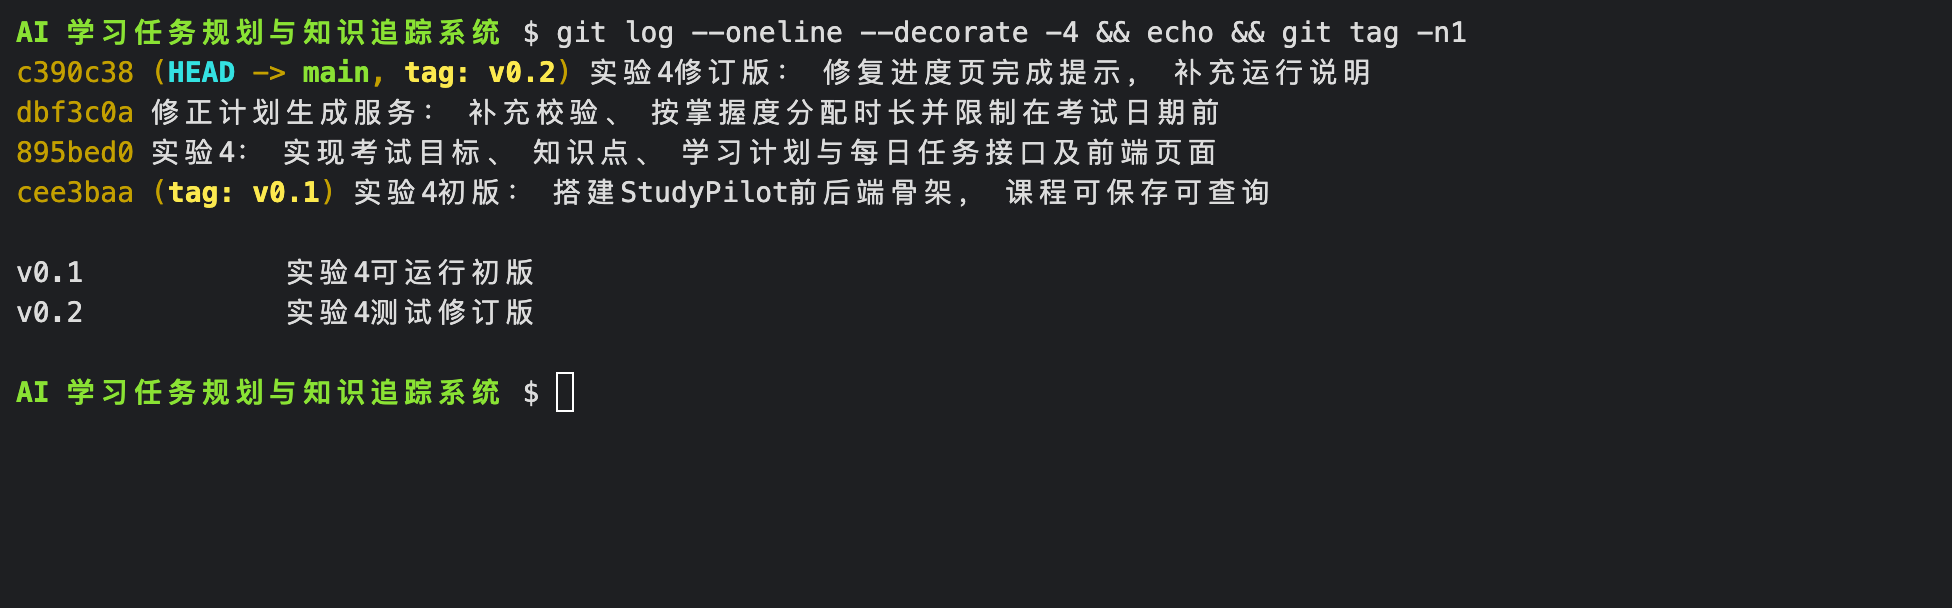
\includegraphics[width=0.94\textwidth]{v02-git-log.png}\label{fig:gitlog}
\caption{两个版本的Commit与Tag记录}
\end{figure}

\begin{figure}[H]
\centering
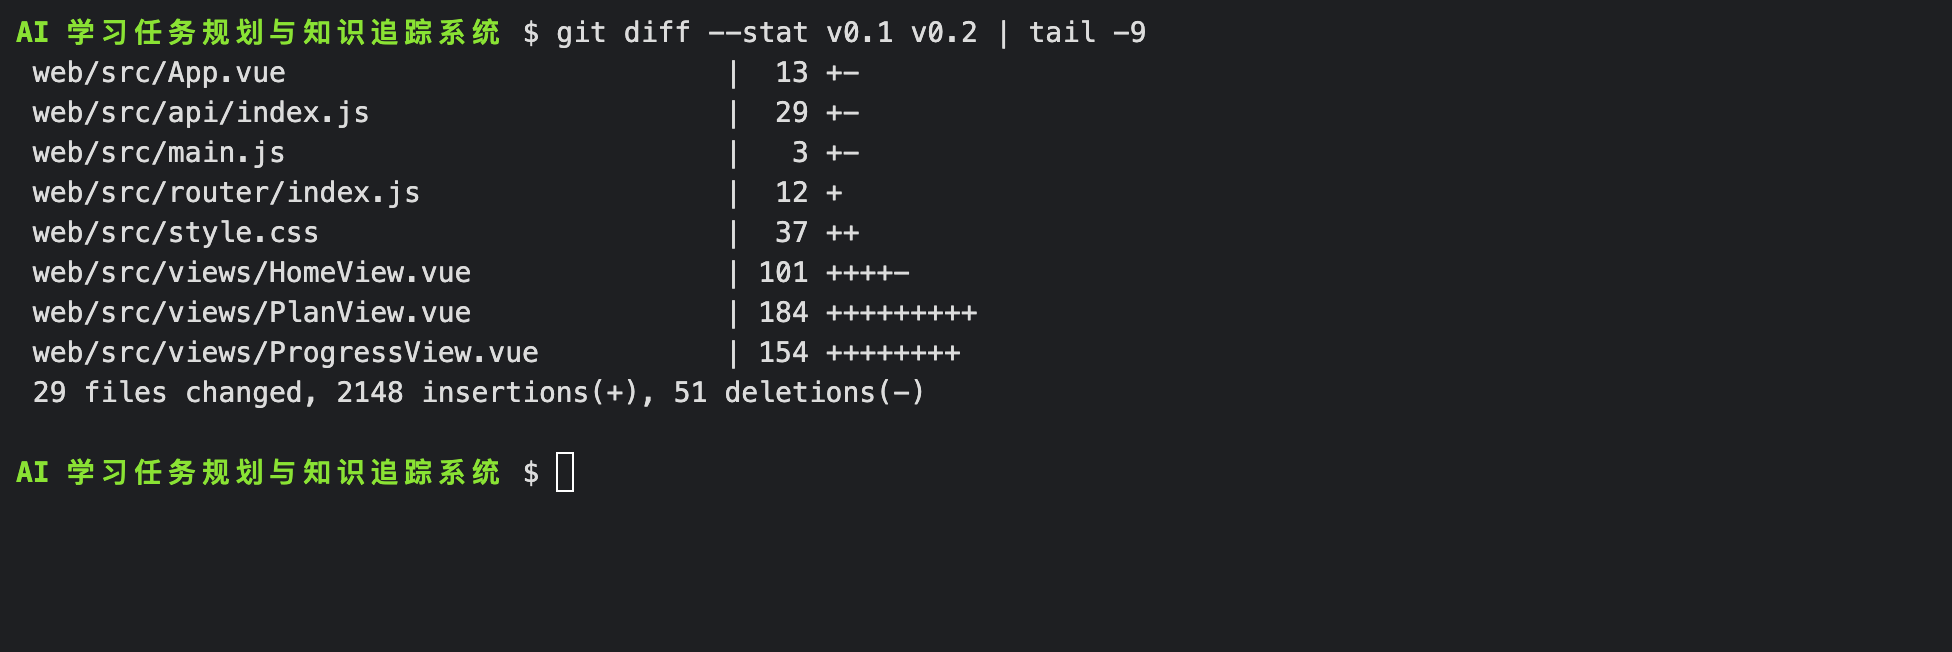
\includegraphics[width=0.94\textwidth]{v02-diff-stat.png}\label{fig:diffstat}
\caption{初版到修订版的文件变化统计}
\end{figure}

两个版本之间的主要变化：新增考试目标、知识点、学习计划和每日任务四组接口，前端从单页改为三个页面；计划生成改为“模型服务不可用就用规则模板”；补上空数据、重复、日期越界等校验；后端增加分层异常处理和日志。

\subsection*{3.2 项目骨架与核心数据}

后端按接口层、业务层、数据访问层组织，前端按页面、路由和接口调用组织，与实验3的架构设计一致。

\begin{table}[H]
\centering
\caption{目录与职责}
\small
\begin{tabularx}{\textwidth}{p{4.3cm}X}
\toprule
目录 & 职责 \\
\midrule
\texttt{backend/app/api} & 接口层，定义路由和输入模型，把请求交给业务层 \\
\texttt{backend/app/service} & 业务层，做字段校验、规则计算和流程控制 \\
\texttt{backend/app/repository} & 数据访问层，负责建表、SQL 执行和数据转换 \\
\texttt{backend/tests} & pytest 测试用例，使用独立的临时数据库 \\
\texttt{backend/seed\_data.json} & 样例数据，由 \texttt{app/seed.py} 读取写入 \\
\texttt{web/src/views} & 首页、学习计划页、学习进度页 \\
\texttt{web/src/api} & 前端接口调用封装，统一处理错误提示 \\
\texttt{web/src/router} & 三个页面之间的路由跳转 \\
\bottomrule
\end{tabularx}
\end{table}

\begin{figure}[H]
\centering
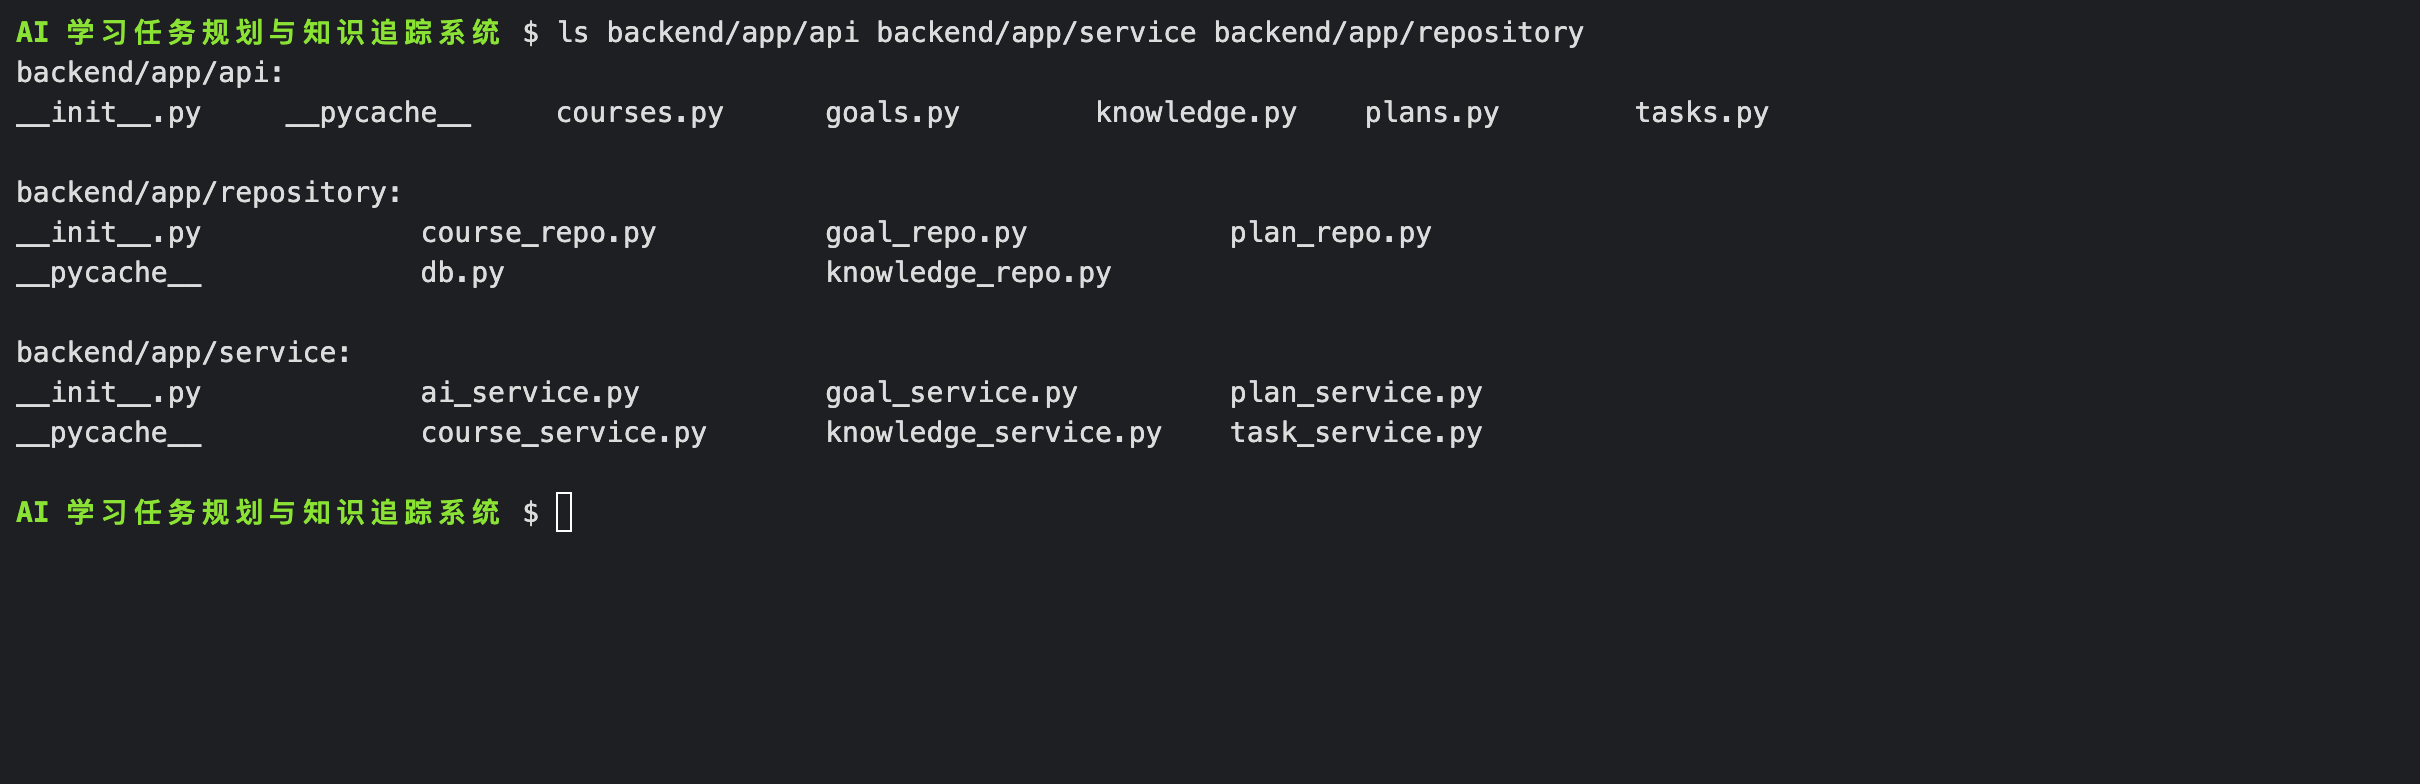
\includegraphics[width=0.92\textwidth]{v02-structure.png}\label{fig:structure}
\caption{后端分层目录}
\end{figure}

\begin{figure}[H]
\centering
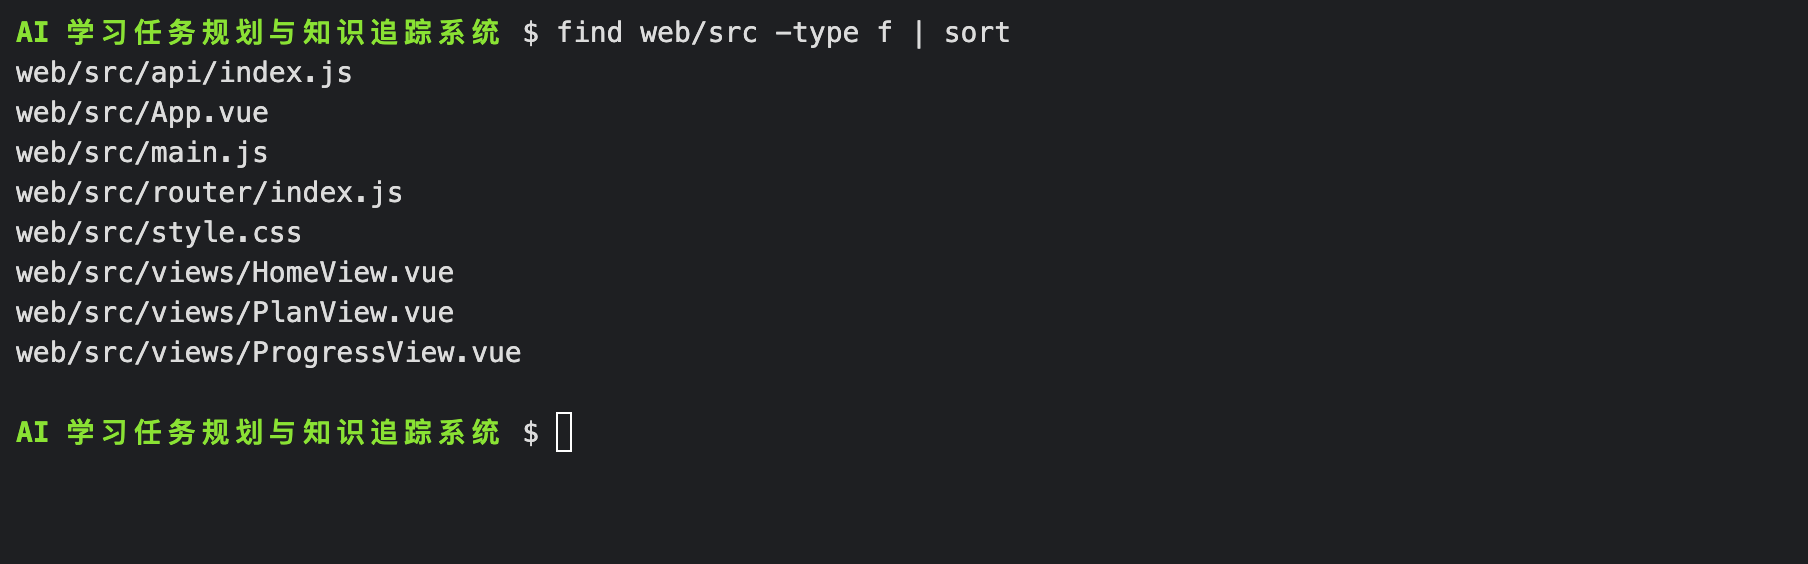
\includegraphics[width=0.92\textwidth]{v02-structure-web.png}\label{fig:structureweb}
\caption{前端目录}
\end{figure}

数据库选择 SQLite：单文件、不需要额外服务，随仓库就能带走，适合个人项目和演示；数据访问使用 Python 标准库 \texttt{sqlite3} 加手写 SQL，方便对照实验3的 ER 图检查字段。启动时执行建表语句并保证存在一个用户，样例数据单独放在 \texttt{seed\_data.json}，用 \texttt{python3 -m app.seed} 写入，\texttt{--clear} 清空，\texttt{--reset} 清空后重新写入。

\begin{figure}[H]
\centering
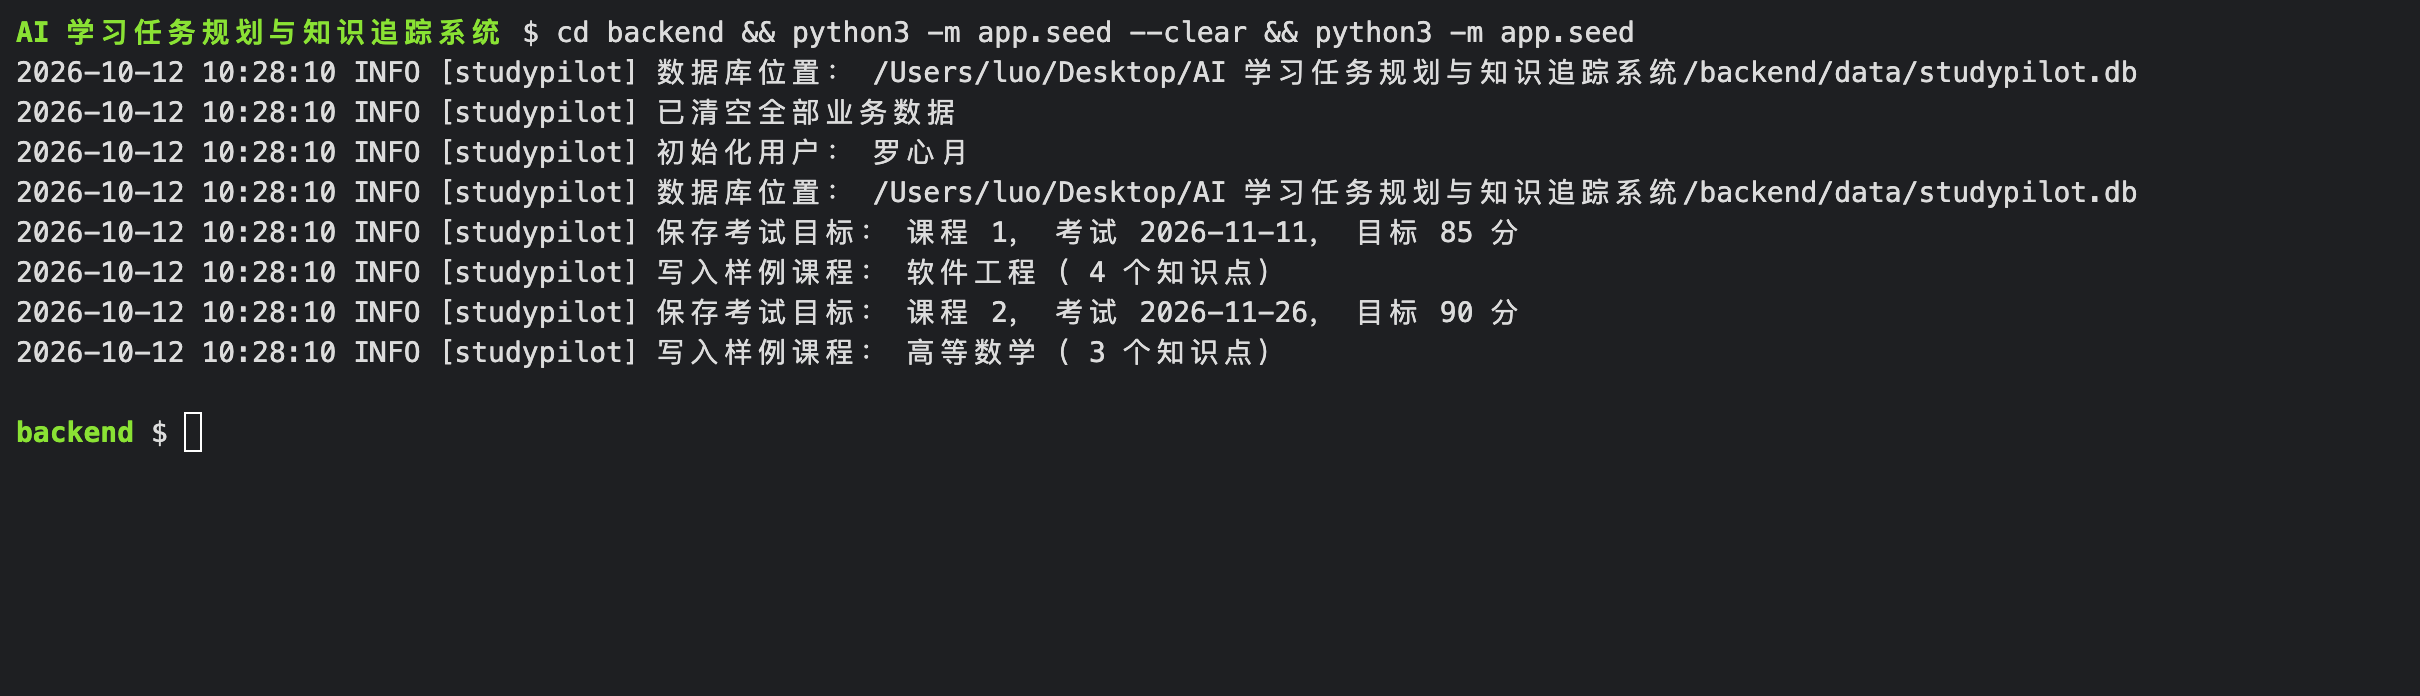
\includegraphics[width=0.96\textwidth]{v02-seed.png}\label{fig:seed}
\caption{样例数据的清空与恢复}
\end{figure}

数据为空、重复、格式错误和读取失败的处理：课程为空时首页显示“还没有课程，先在下面创建一门课程”；课程名或知识点名重复时返回 409；考试日期格式错误或早于今天返回 400；数据库文件损坏时返回 500 并写日志，页面显示“数据库暂时不可用，请稍后重试”。这些情况都在 3.5 的测试里验证。

\subsection*{3.3 主要页面、接口与数据交互}

页面通过 \texttt{fetch} 调用后端接口，接口返回统一结构，出错时带 \texttt{code} 和 \texttt{message}，页面直接把 \texttt{message} 显示给用户。

\begin{table}[H]
\centering
\caption{主要接口}
\footnotesize
\begin{tabularx}{\textwidth}{p{5.8cm}X p{4.0cm}}
\toprule
接口 & 输入与输出 & 校验与失败情况 \\
\midrule
POST /api/courses & 名称、学期 → 课程 & 名称为空 400，重名 409 \\
POST /api/courses/\{id\}/goal & 考试日期、目标分、每天可用分钟 → 考试目标 & 日期早于今天或格式错误 400 \\
POST /api/courses/\{id\}/points & 知识点名称、掌握度 → 知识点 & 名称为空 400，重名 409，掌握度超范围 422 \\
POST /api/plans/generate & 课程编号 → 候选任务列表 & 没有考试目标 400，没有知识点 400，考试前无可用日期 400 \\
POST /api/plans/confirm & 课程编号、任务列表 → 计划编号 & 任务为空 400，任务日期晚于考试 400 \\
POST /api/tasks/\{id\}/complete & 掌握度、备注 → 处理结果 & 任务不存在 404，重复提交 409 \\
\bottomrule
\end{tabularx}
\end{table}

\begin{figure}[H]
\centering
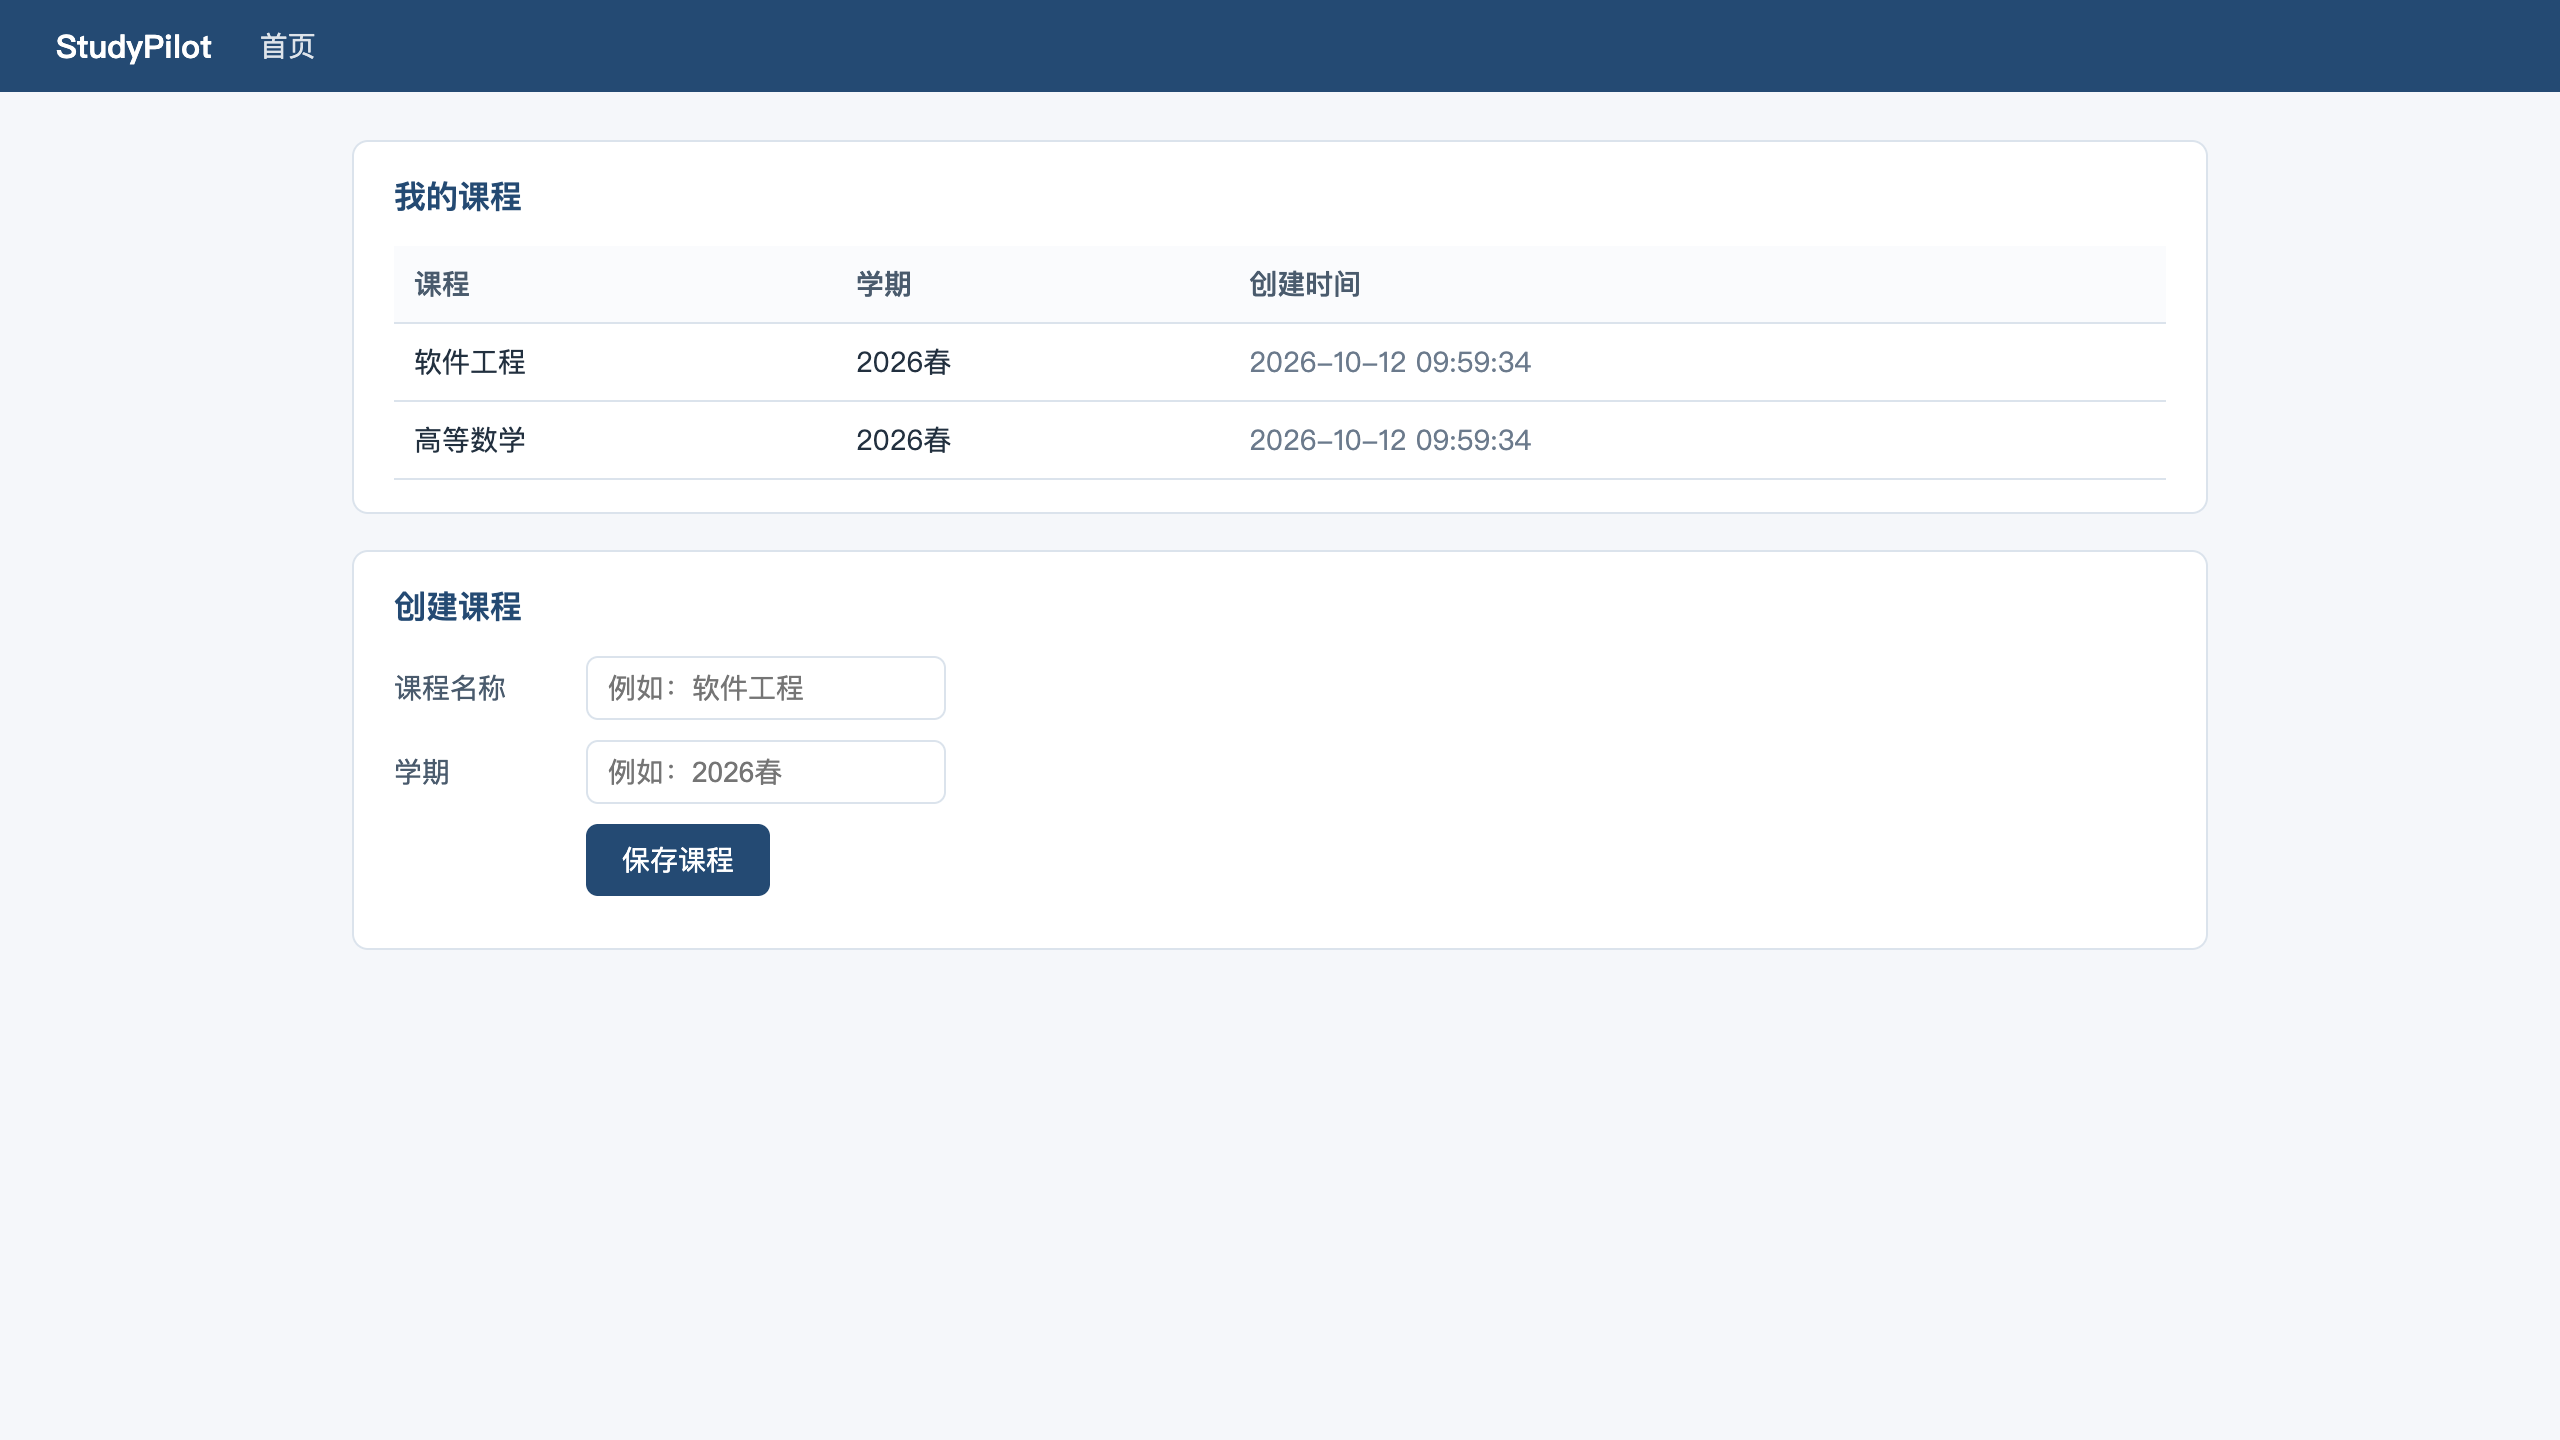
\includegraphics[width=0.86\textwidth]{v01-home.png}\label{fig:v01home}
\caption{初版首页：课程列表与创建课程}
\end{figure}

\begin{figure}[H]
\centering
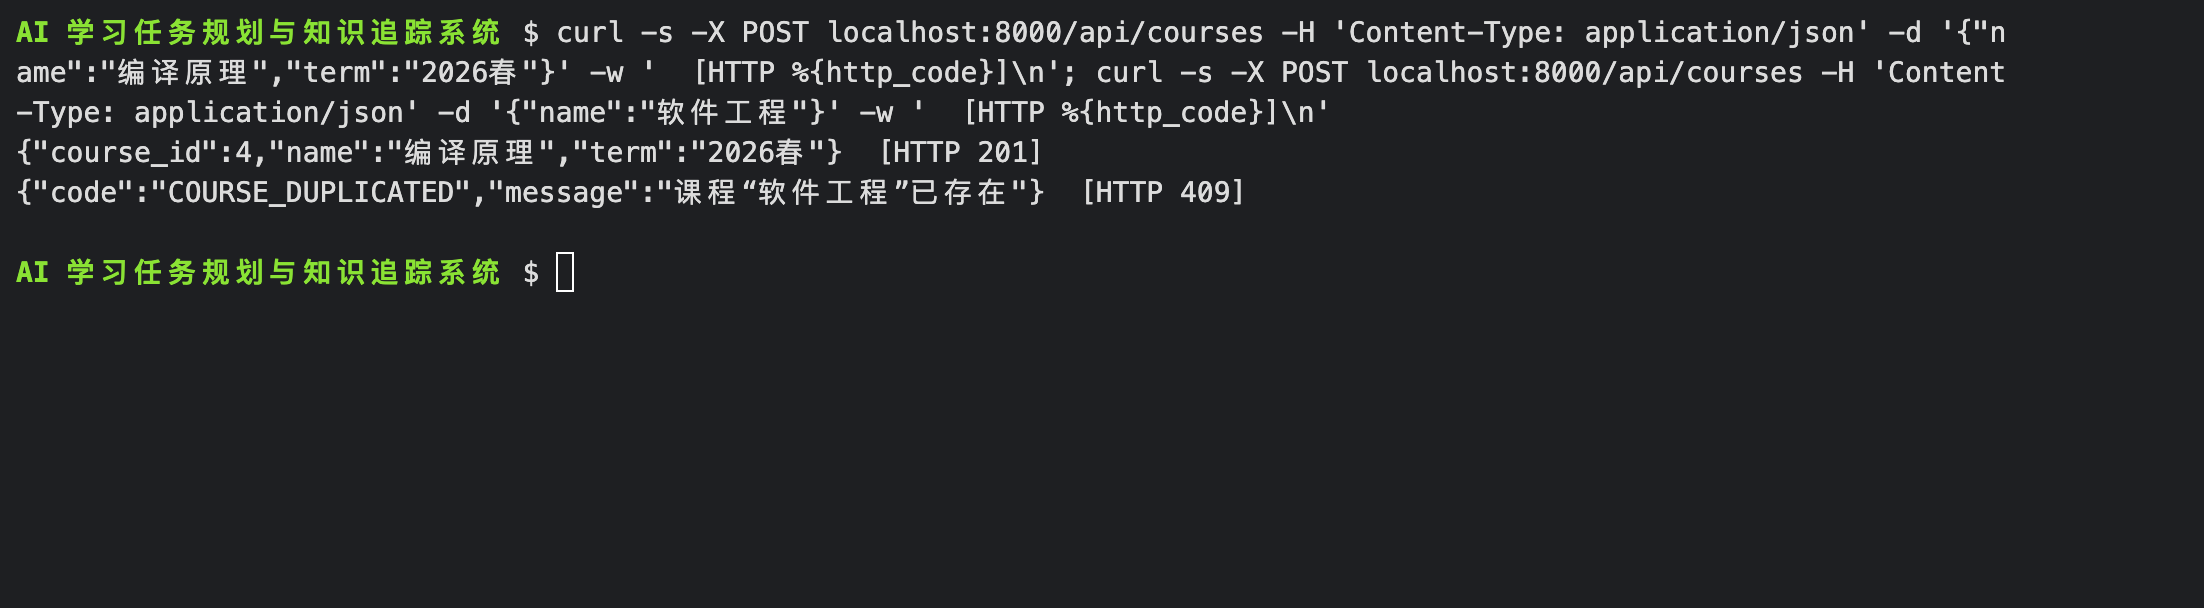
\includegraphics[width=0.96\textwidth]{v01-api.png}\label{fig:v01api}
\caption{初版接口：正常创建返回201，重复课程返回409}
\end{figure}

\begin{figure}[H]
\centering
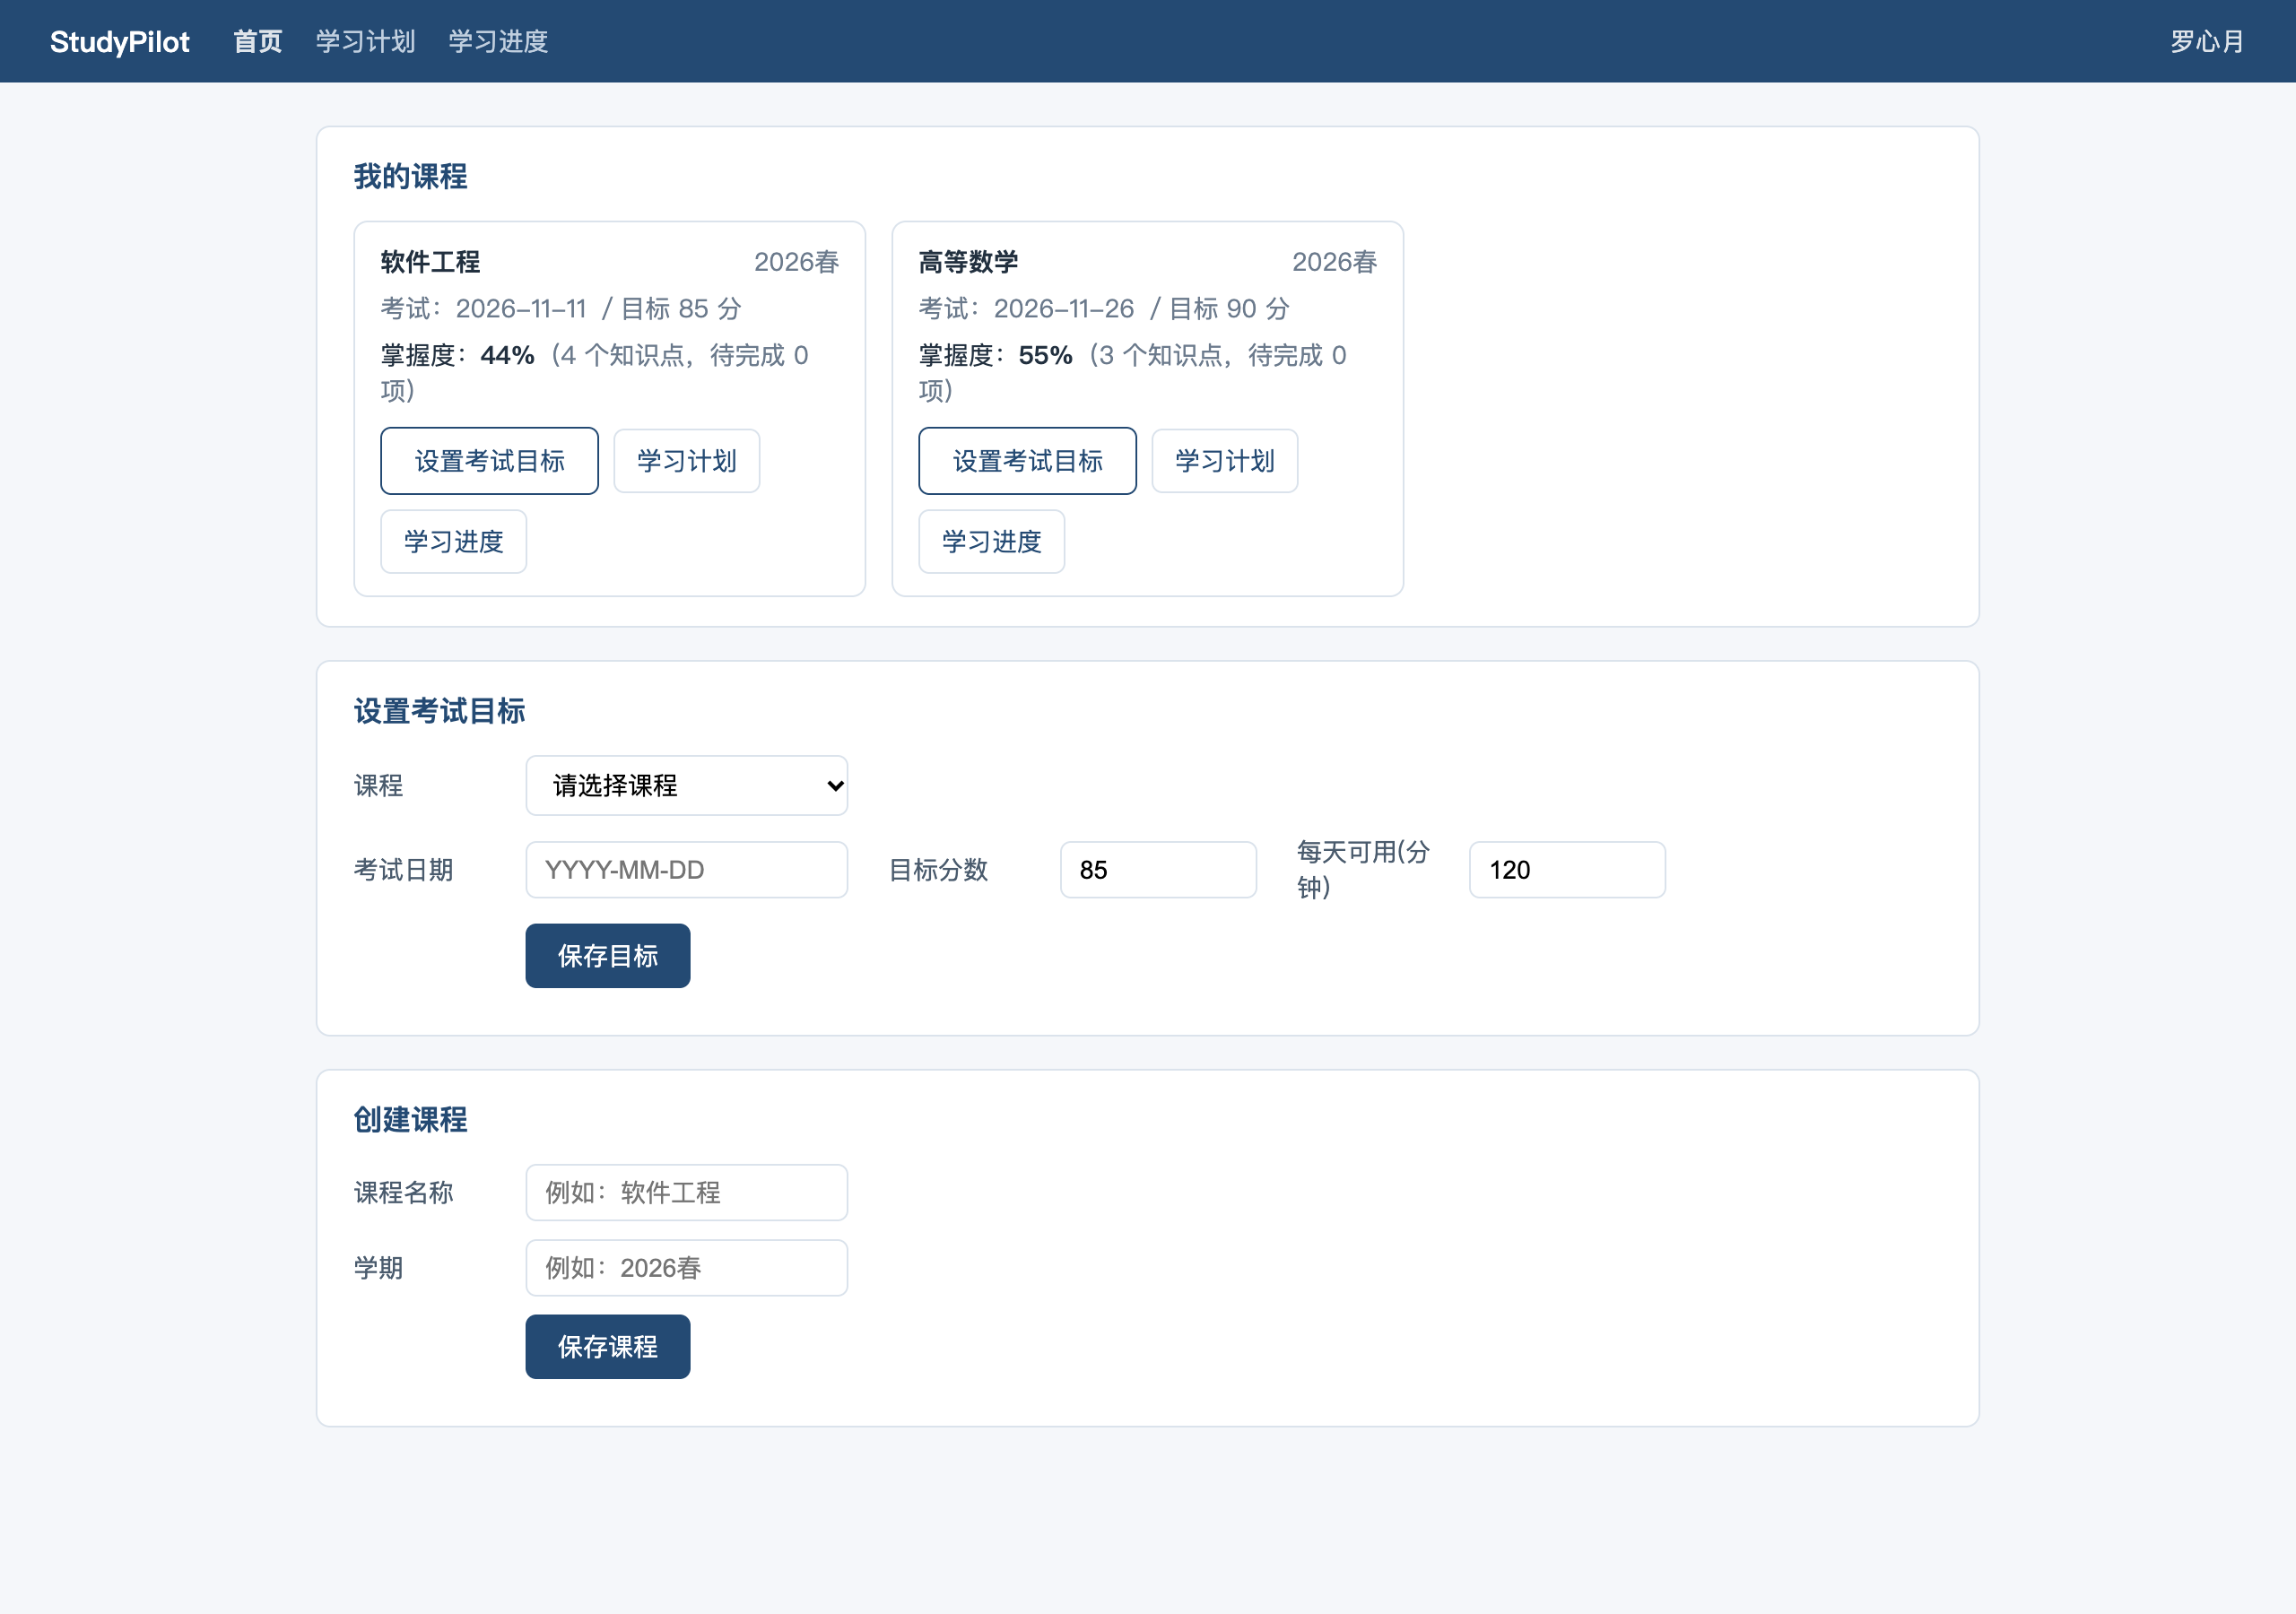
\includegraphics[width=0.88\textwidth]{v02-home.png}\label{fig:home}
\caption{修订版首页：课程、考试目标和掌握度}
\end{figure}

\begin{figure}[H]
\centering
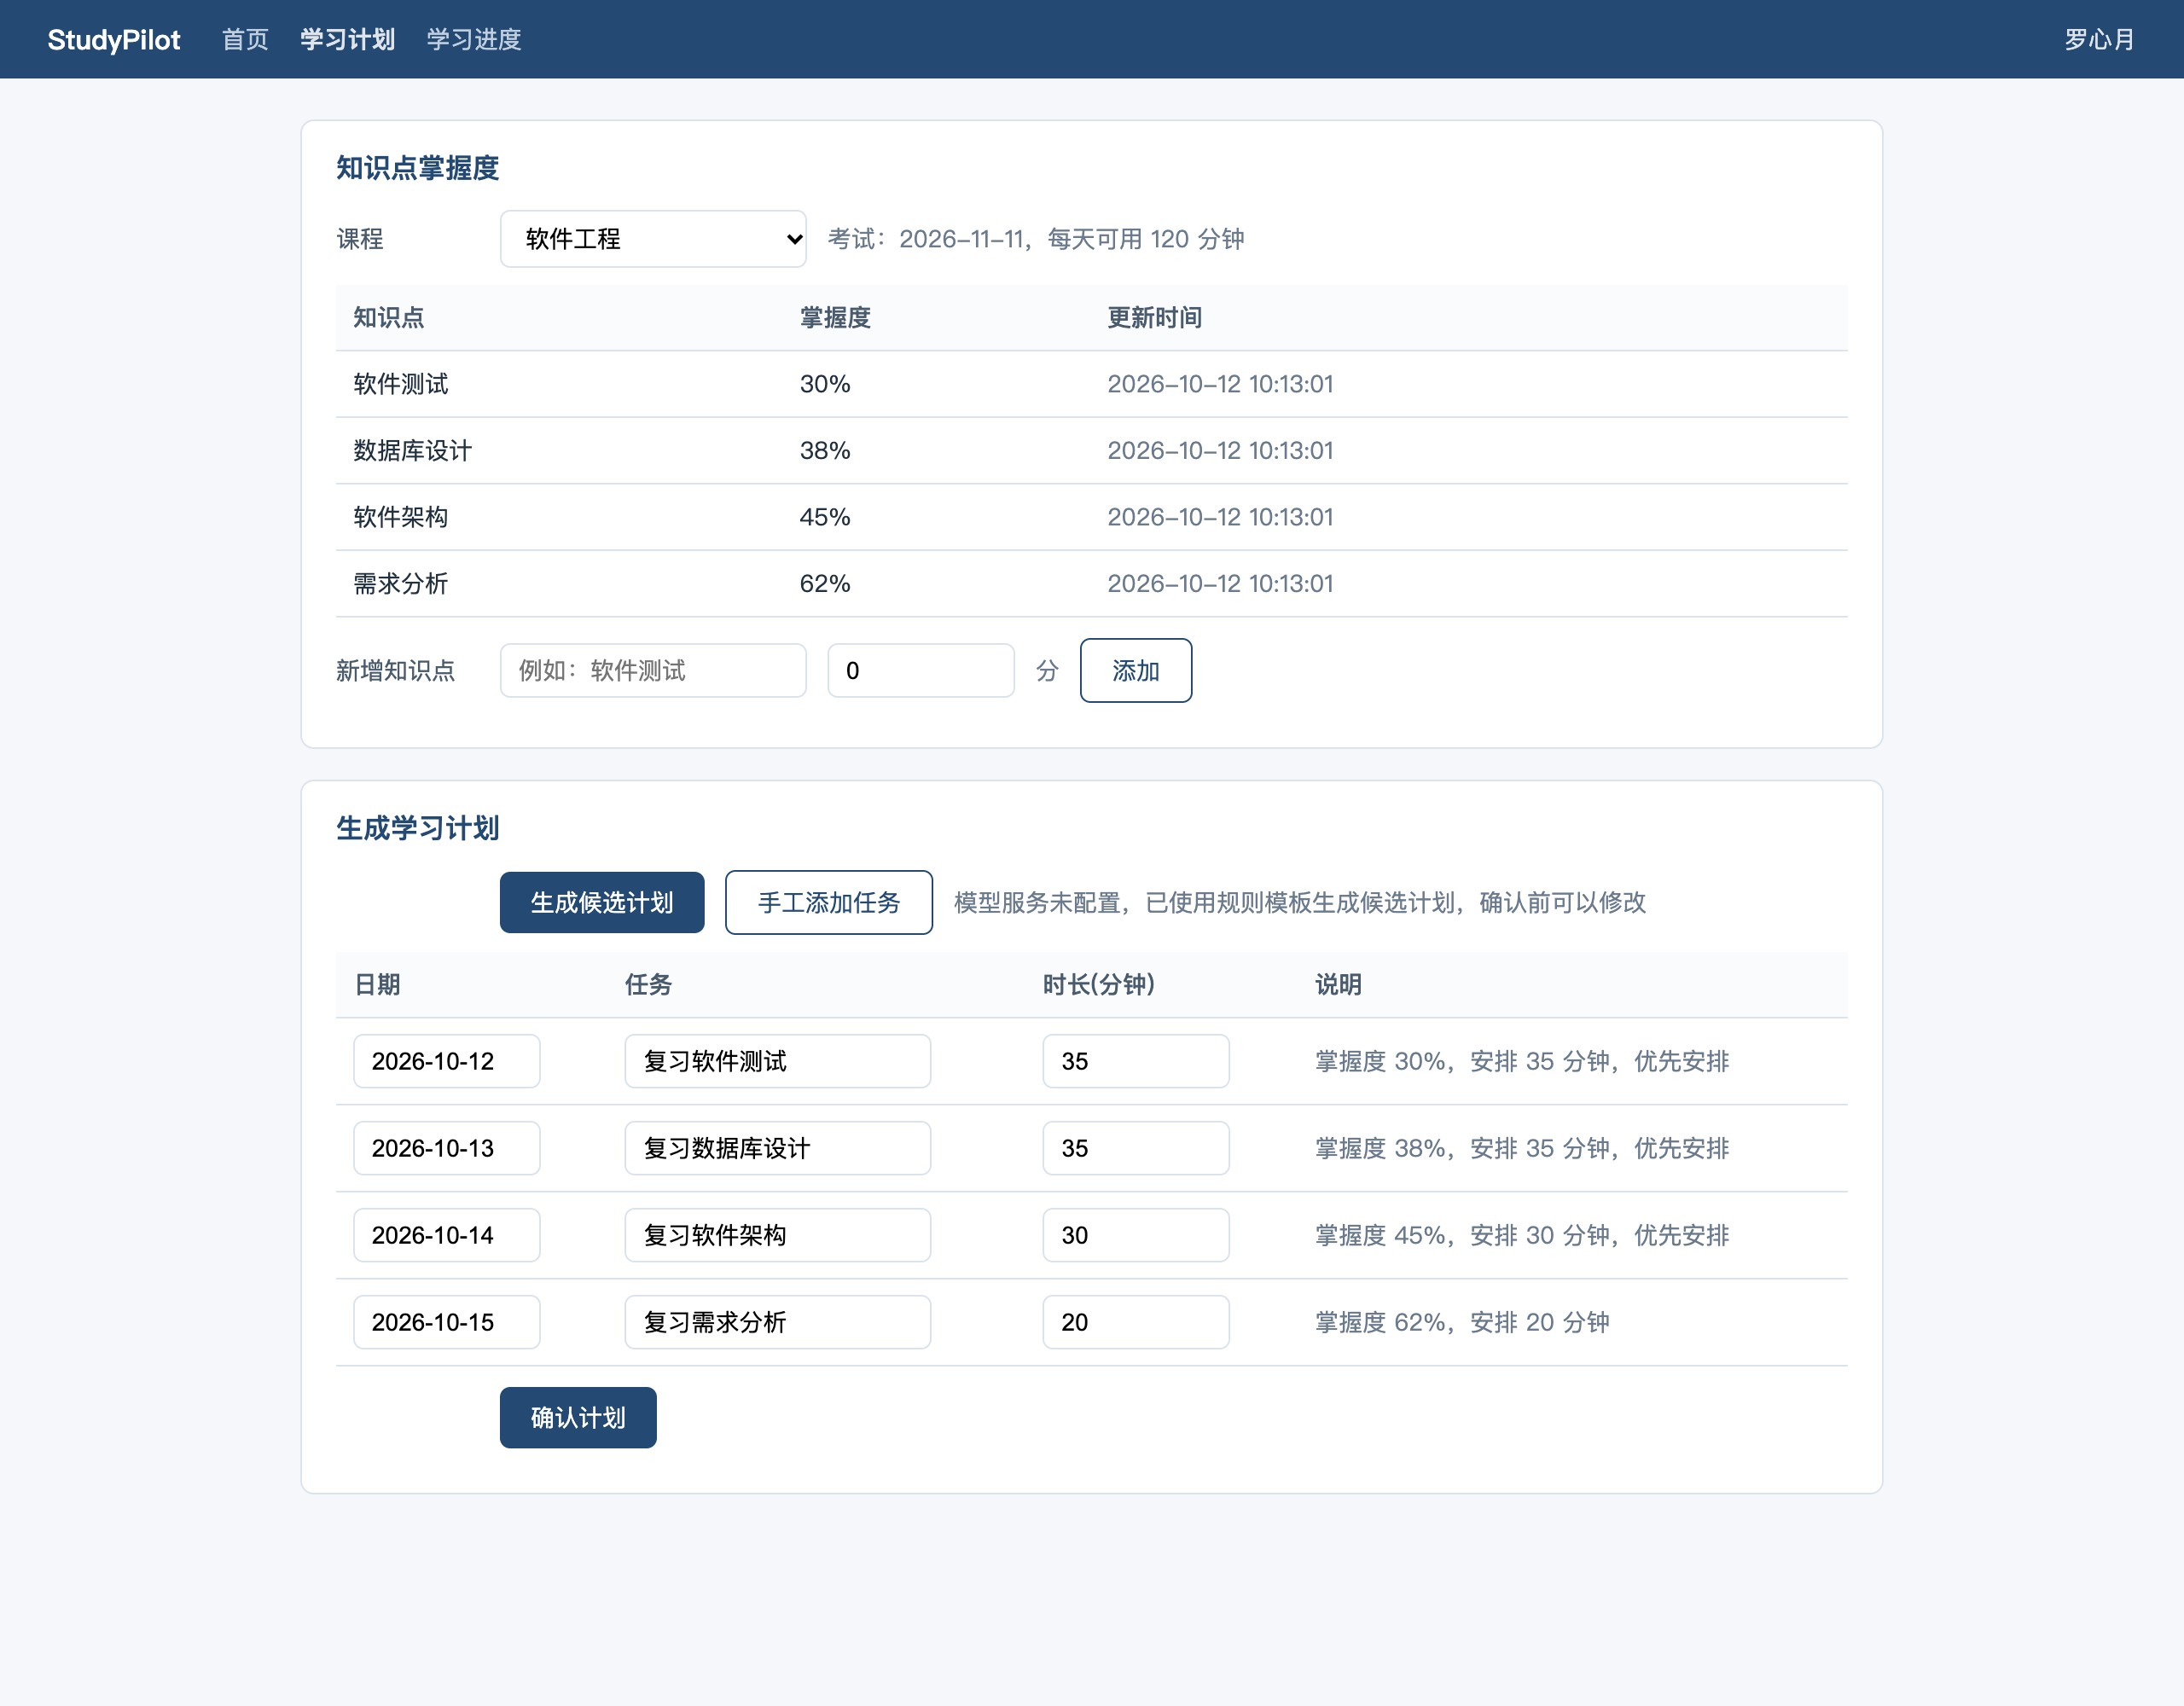
\includegraphics[width=0.88\textwidth]{v02-plan-generate.png}\label{fig:generate}
\caption{生成候选计划：按掌握度分配时长并分散到不同日期}
\end{figure}

\begin{figure}[H]
\centering
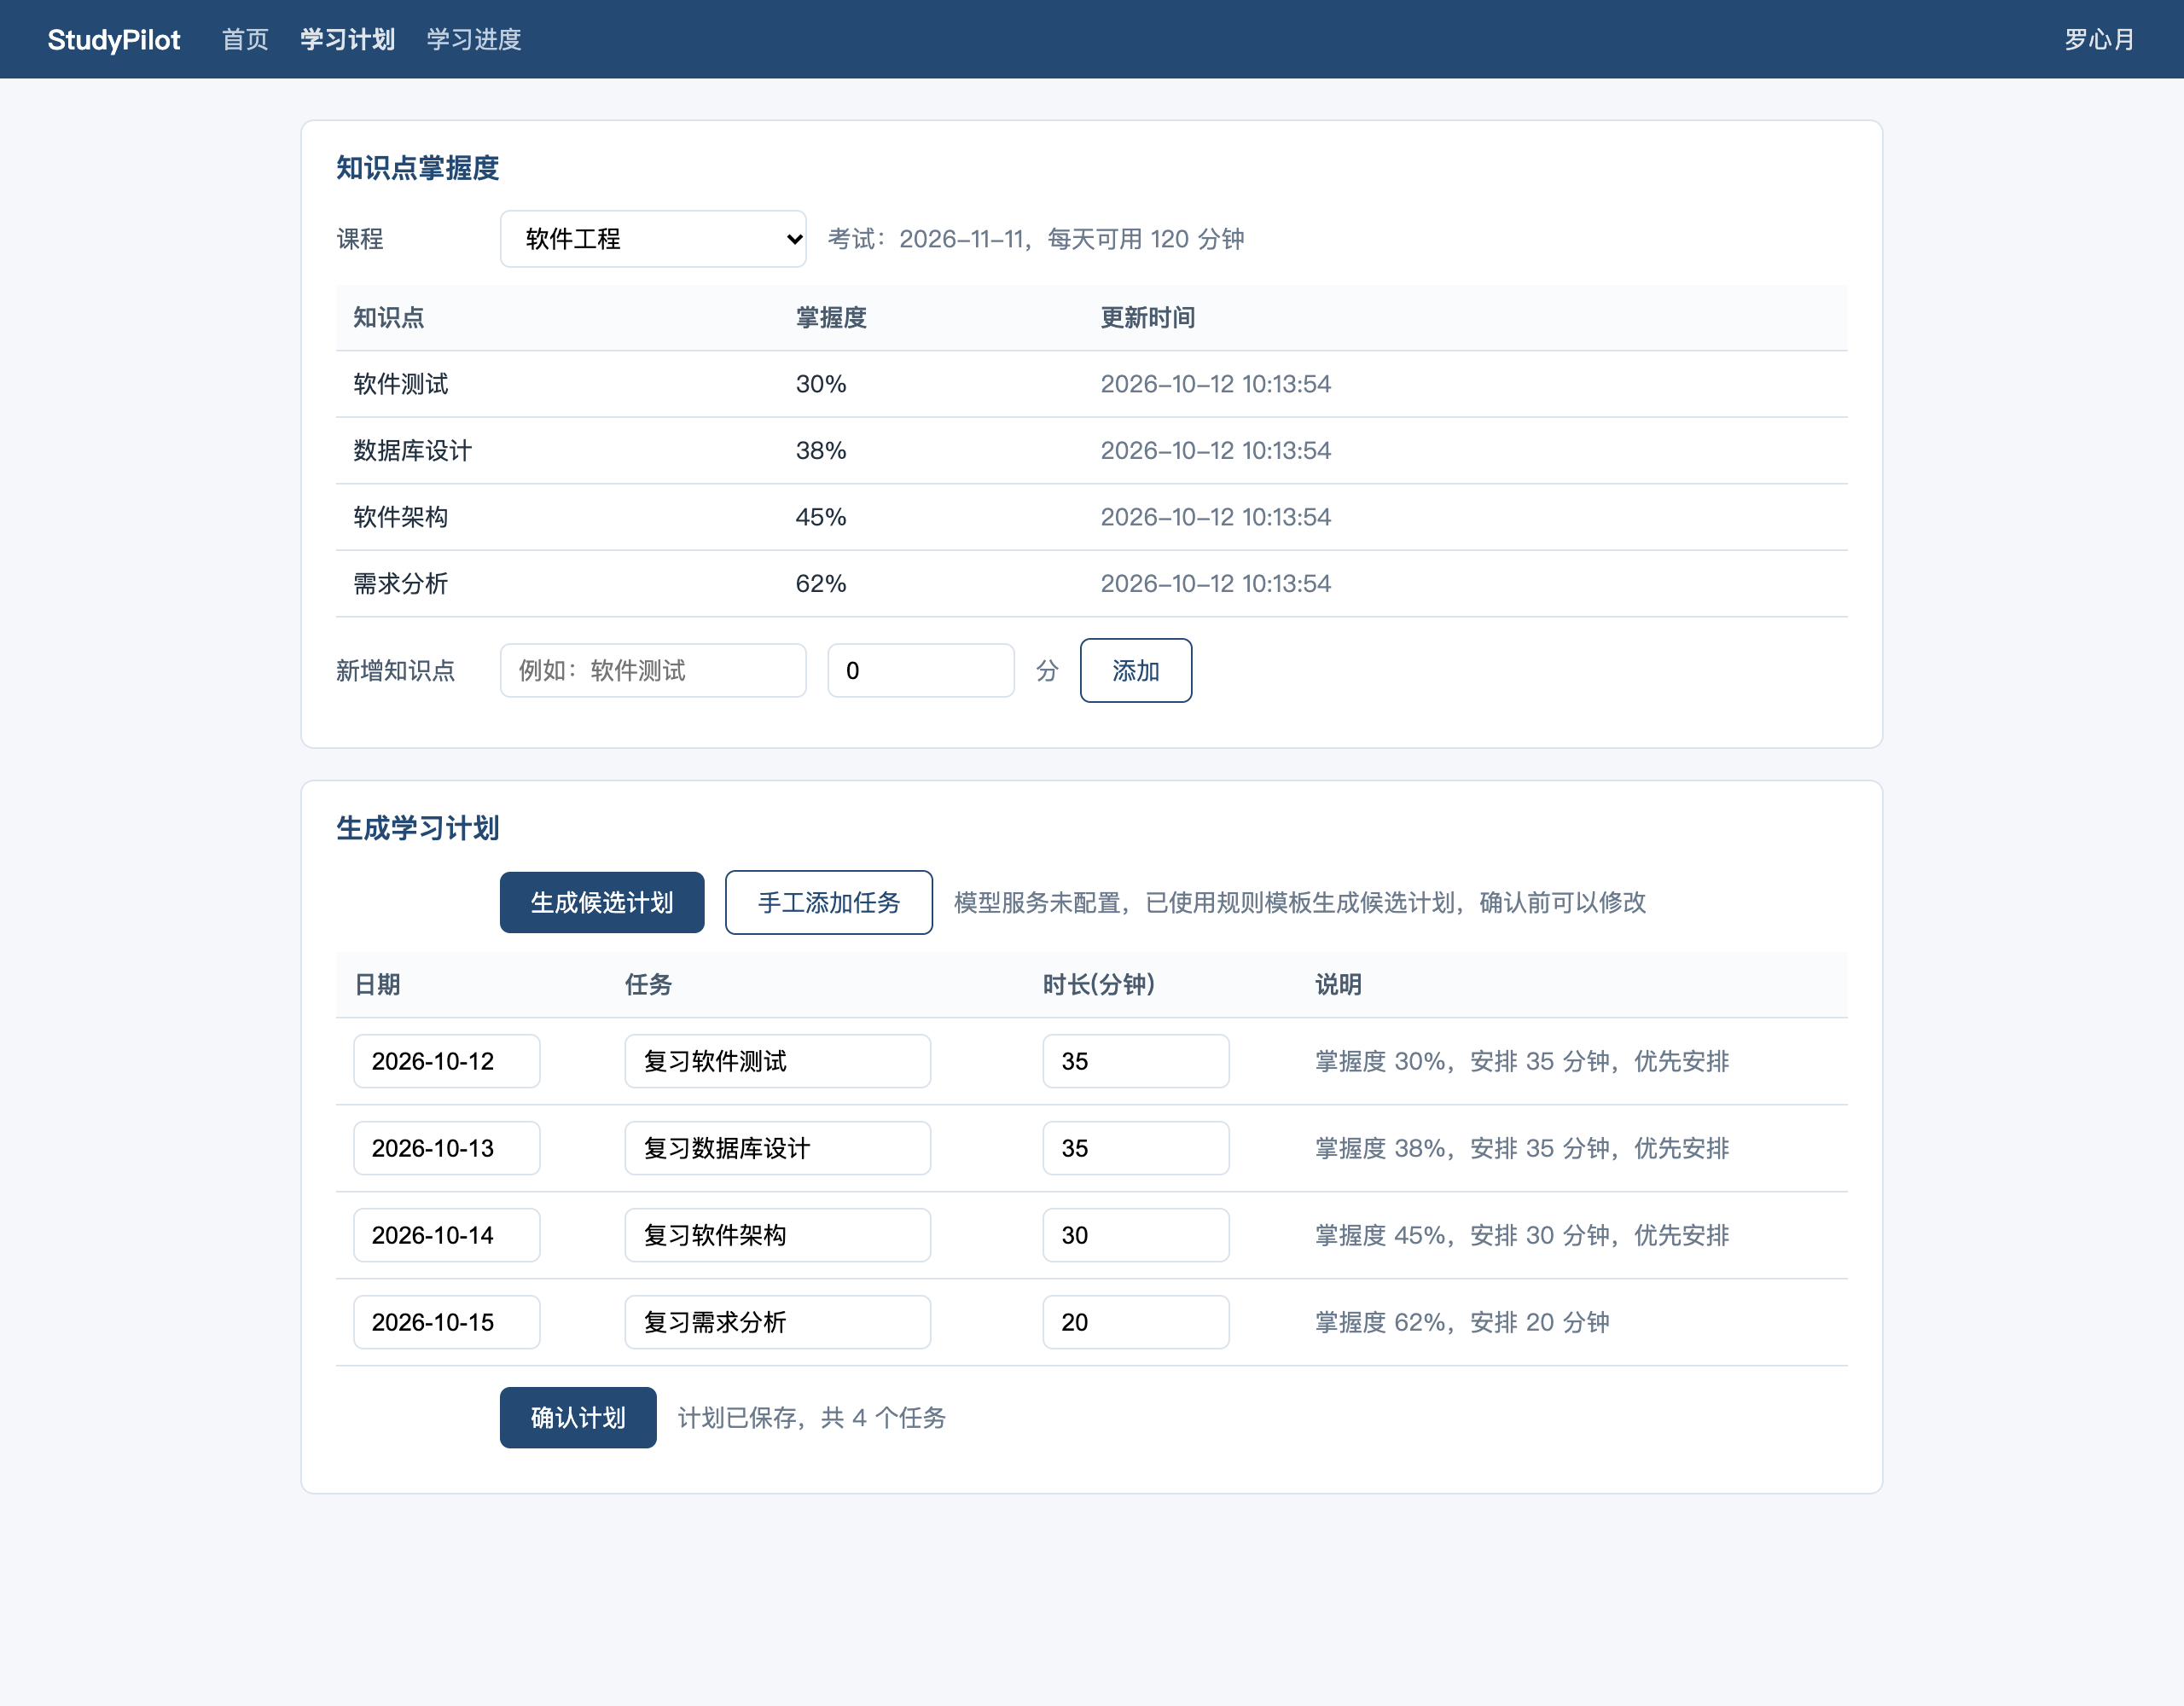
\includegraphics[width=0.88\textwidth]{v02-plan-confirm.png}\label{fig:confirm}
\caption{确认计划后提示已保存的任务数量}
\end{figure}

\begin{figure}[H]
\centering
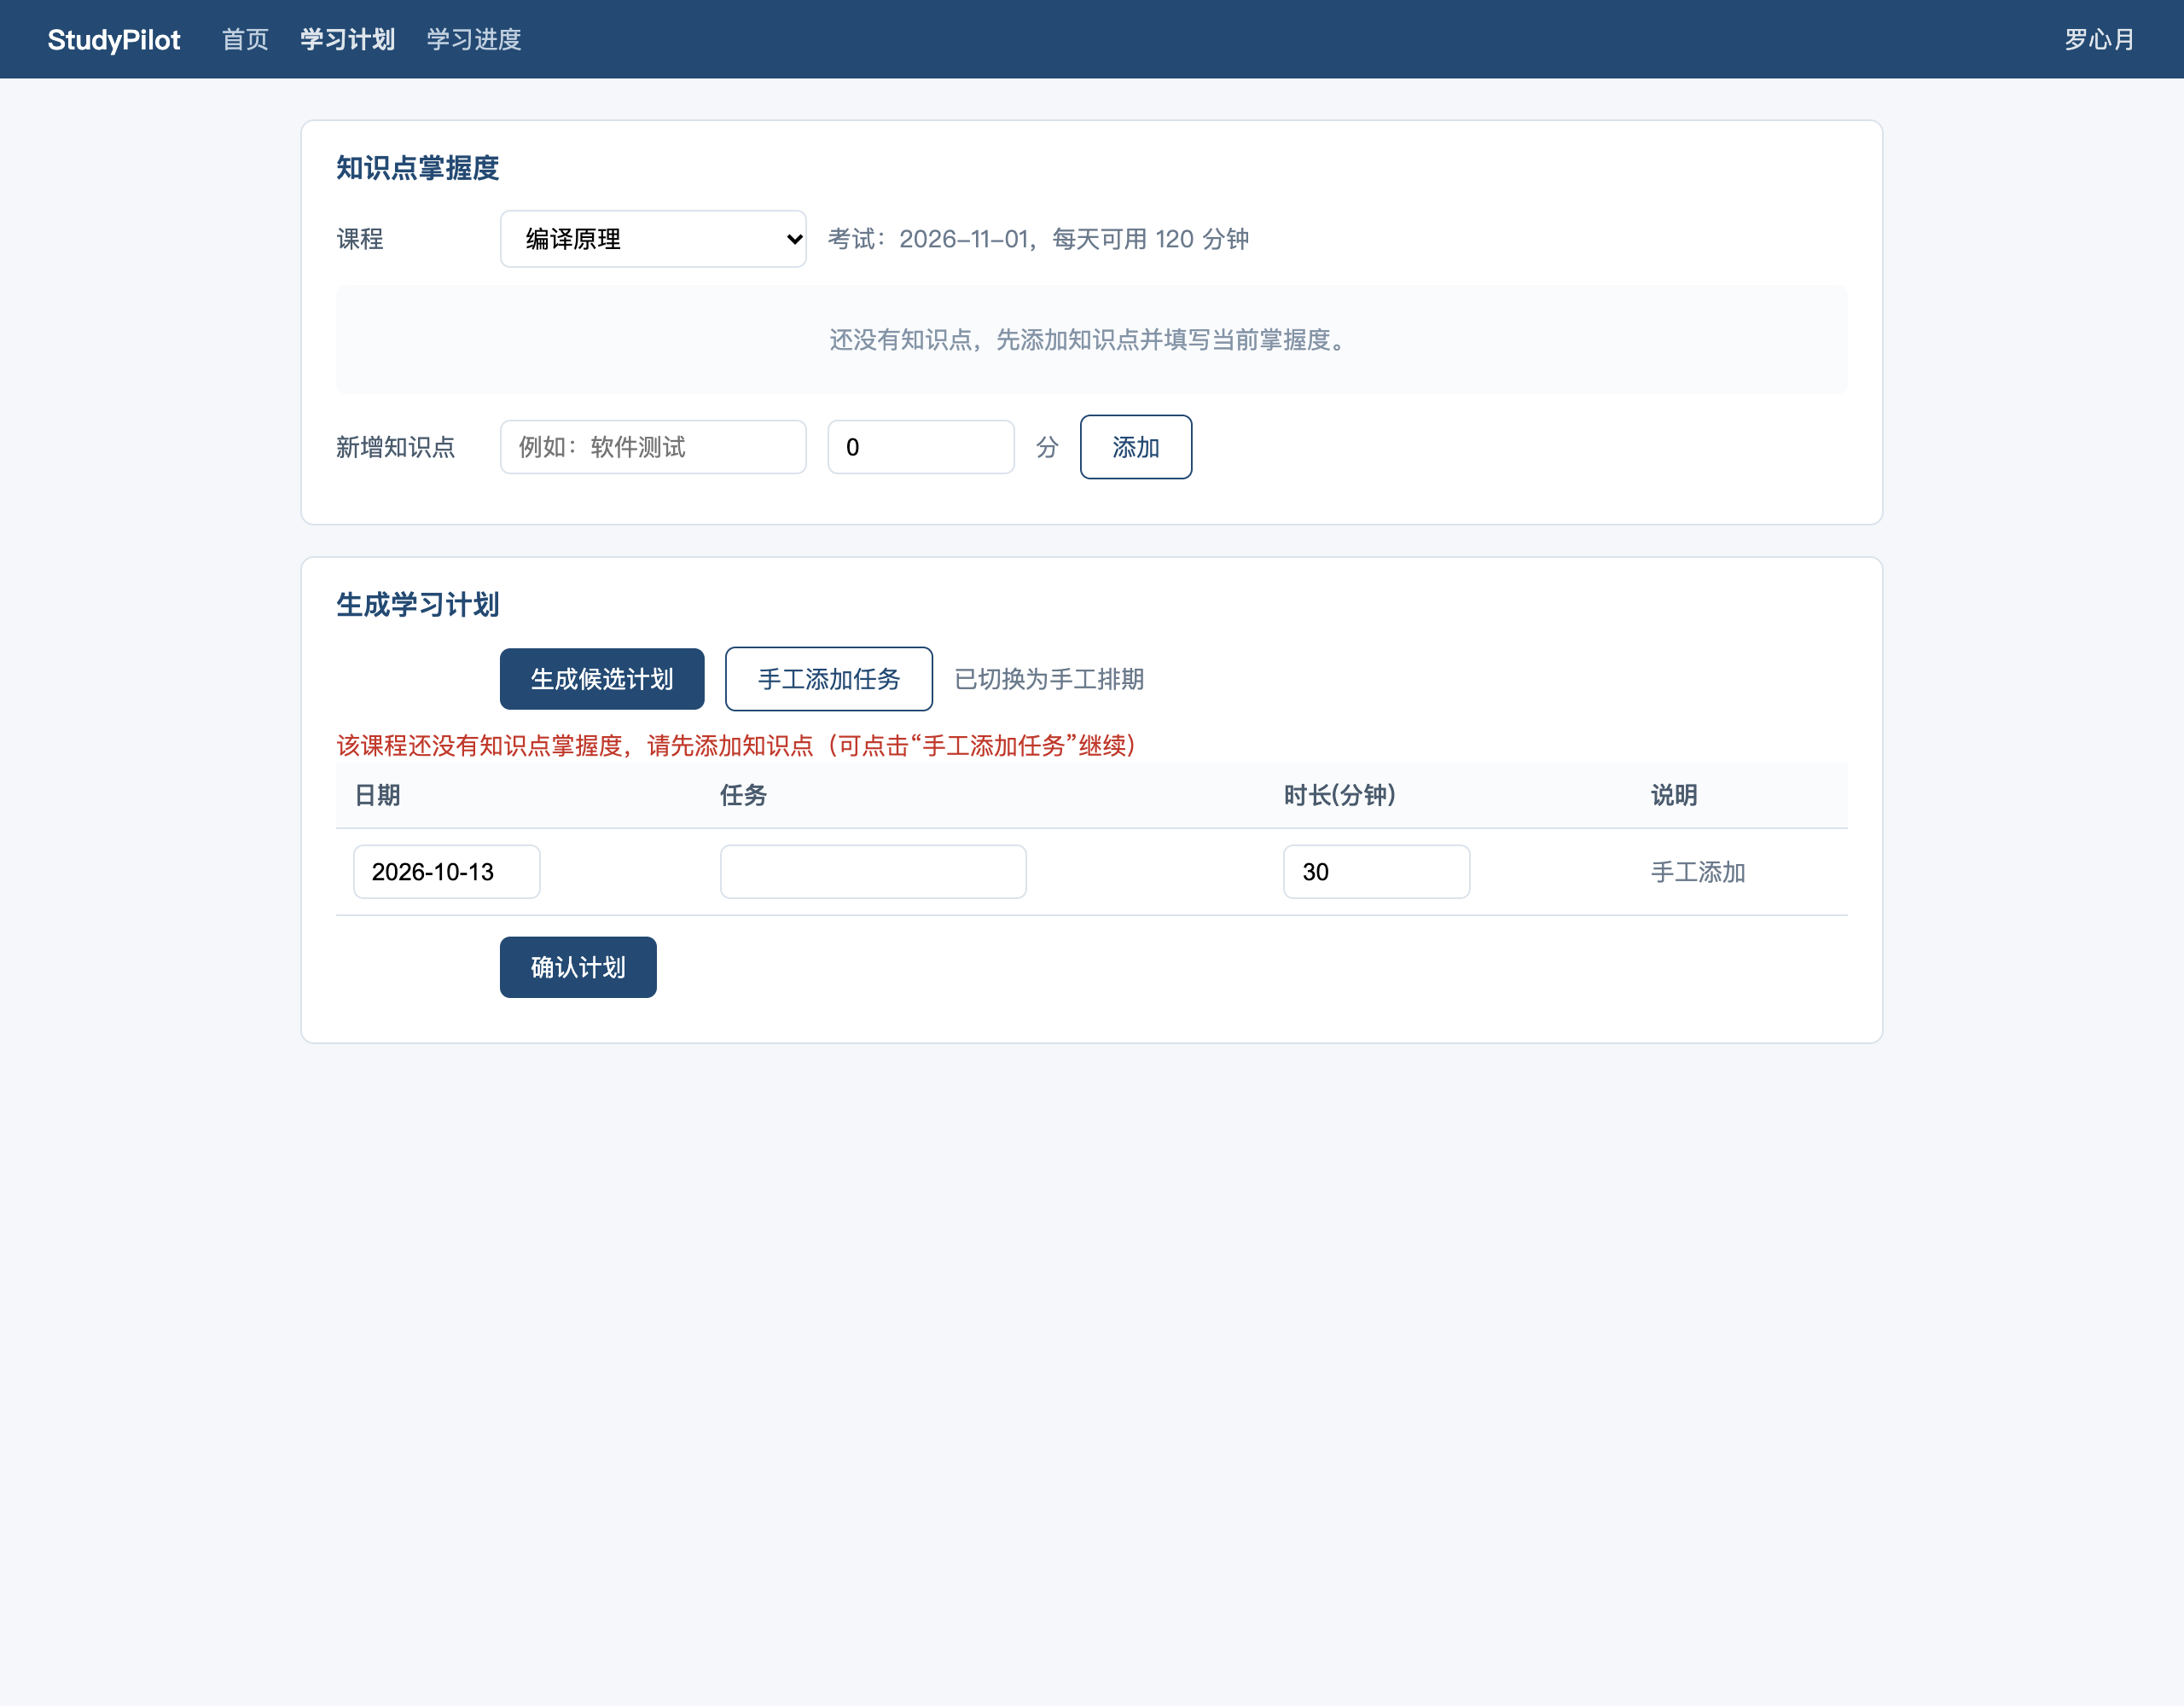
\includegraphics[width=0.88\textwidth]{v02-plan-empty.png}\label{fig:empty}
\caption{空数据反馈：没有知识点时给出提示并保留手工添加入口}
\end{figure}

\begin{figure}[H]
\centering
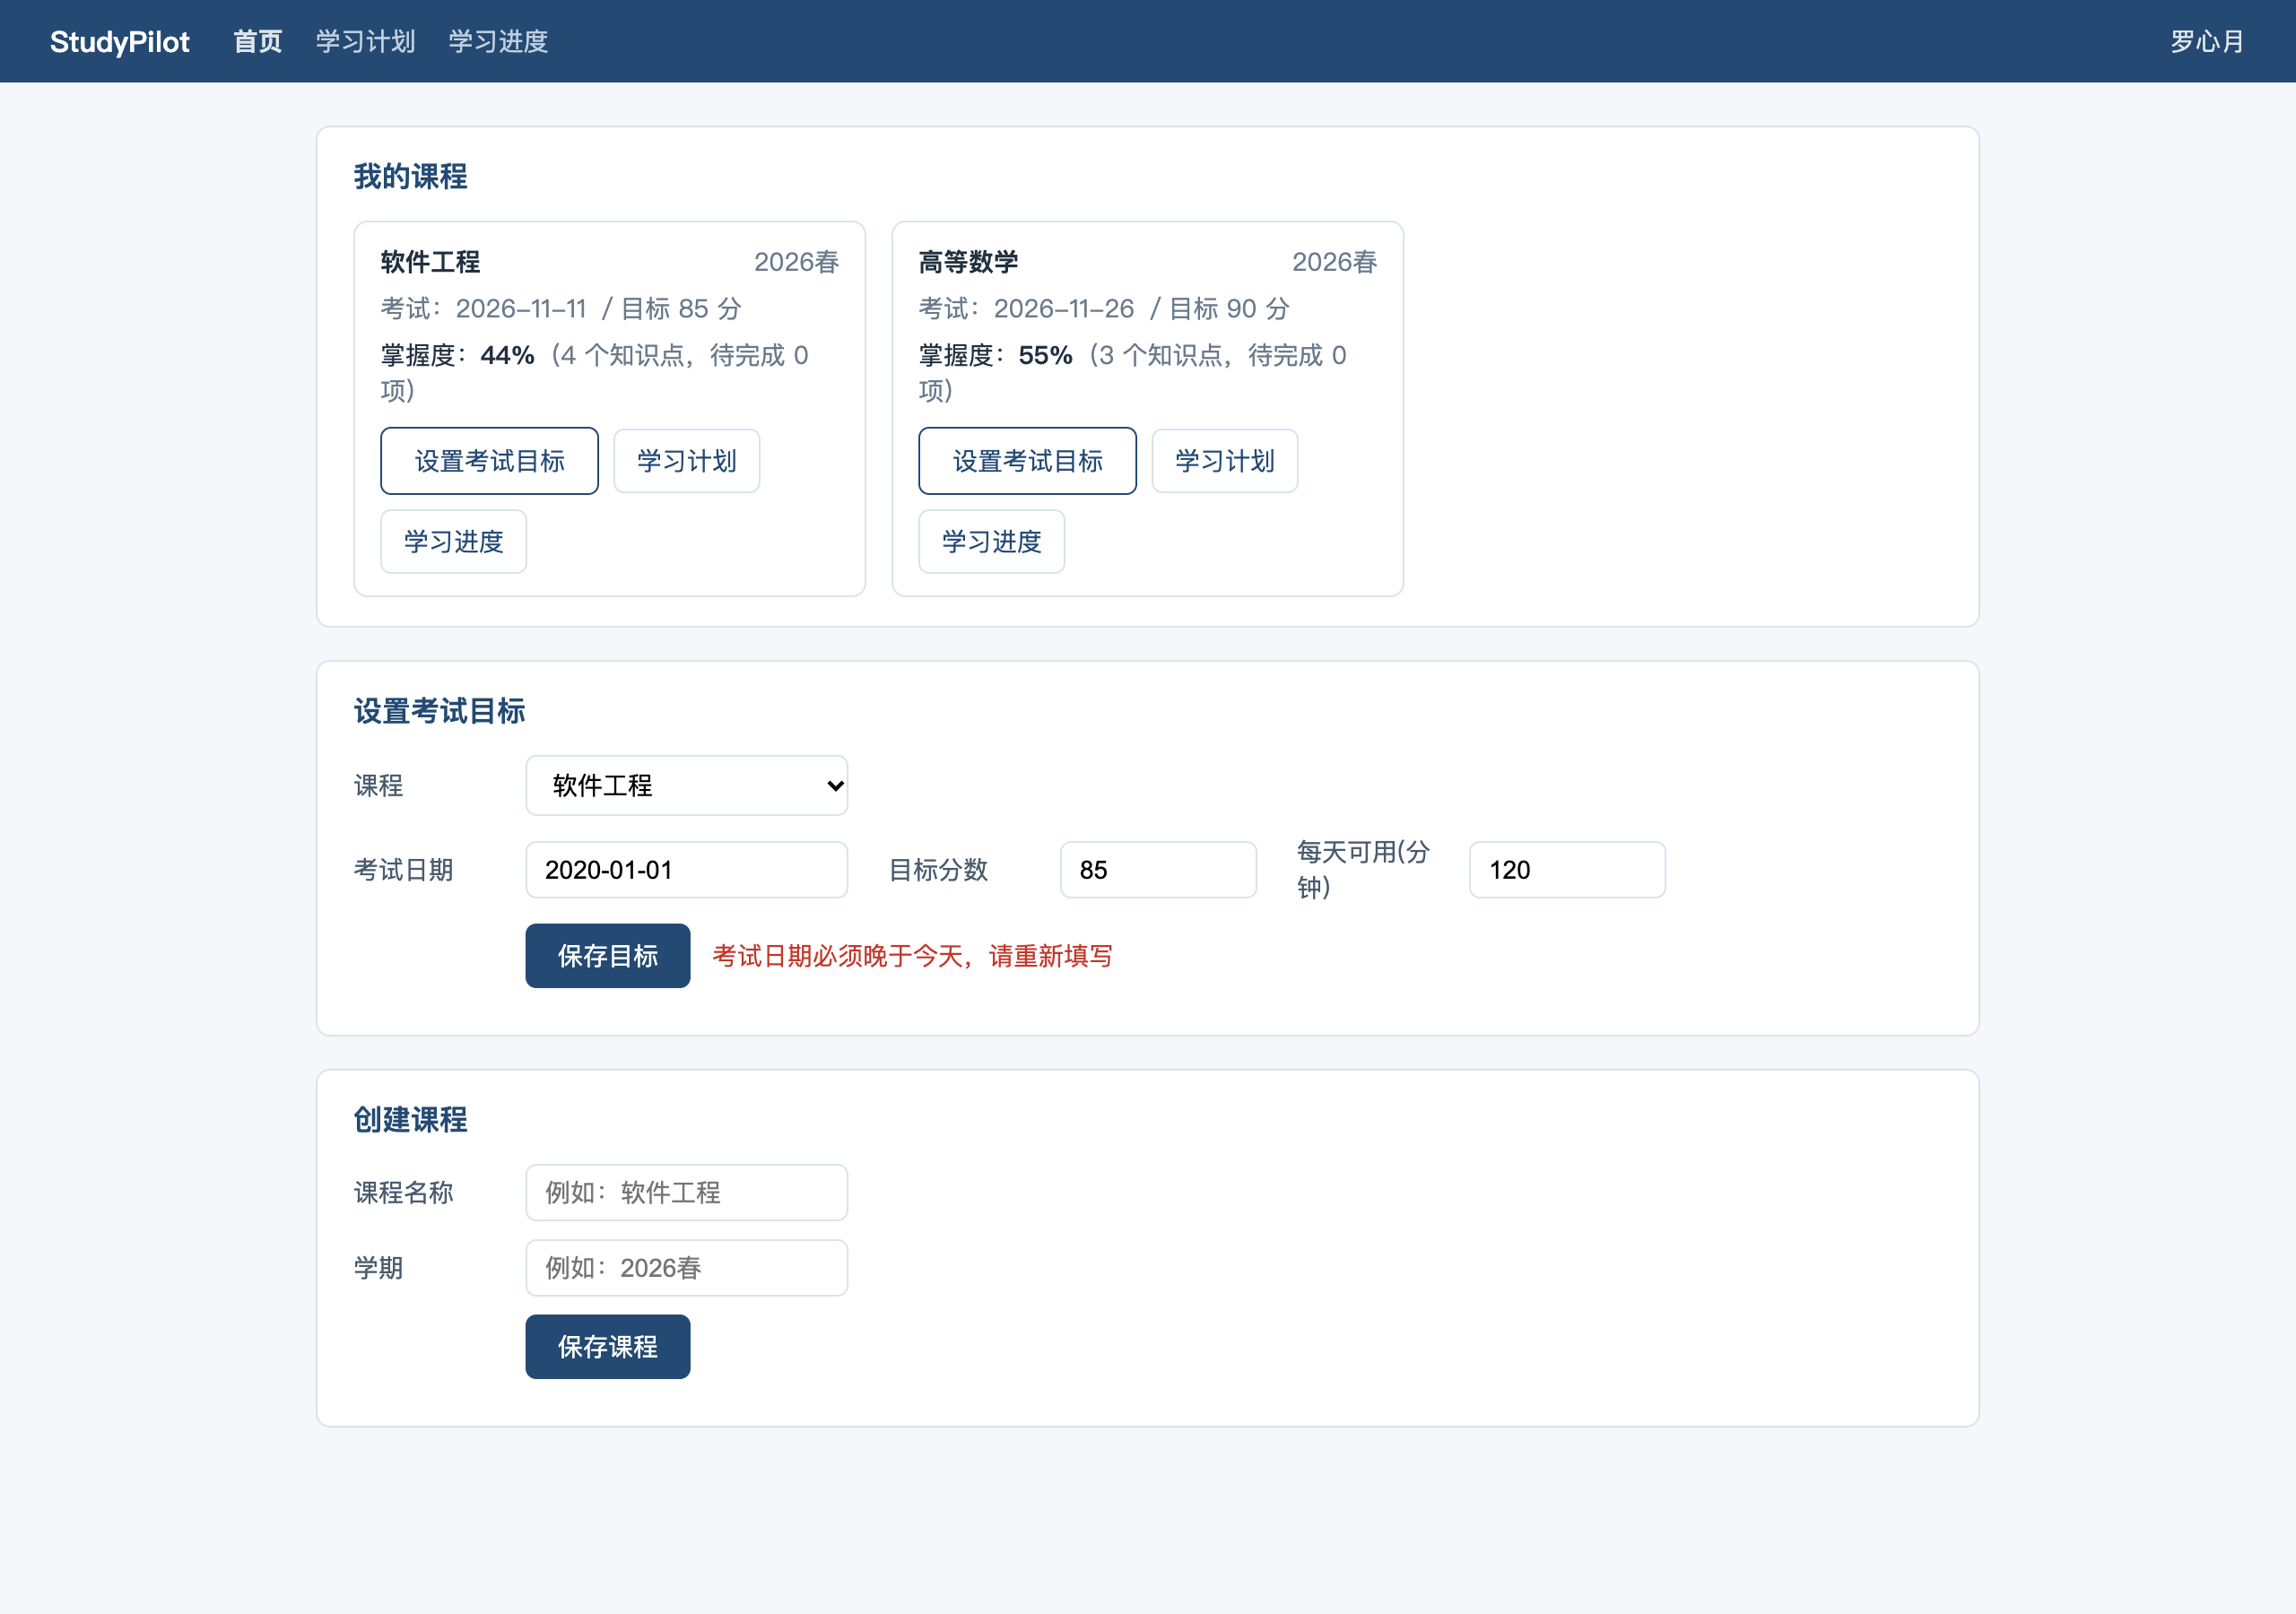
\includegraphics[width=0.88\textwidth]{v02-goal-error.png}\label{fig:goalerror}
\caption{错误输入反馈：考试日期早于今天}
\end{figure}

\begin{figure}[H]
\centering
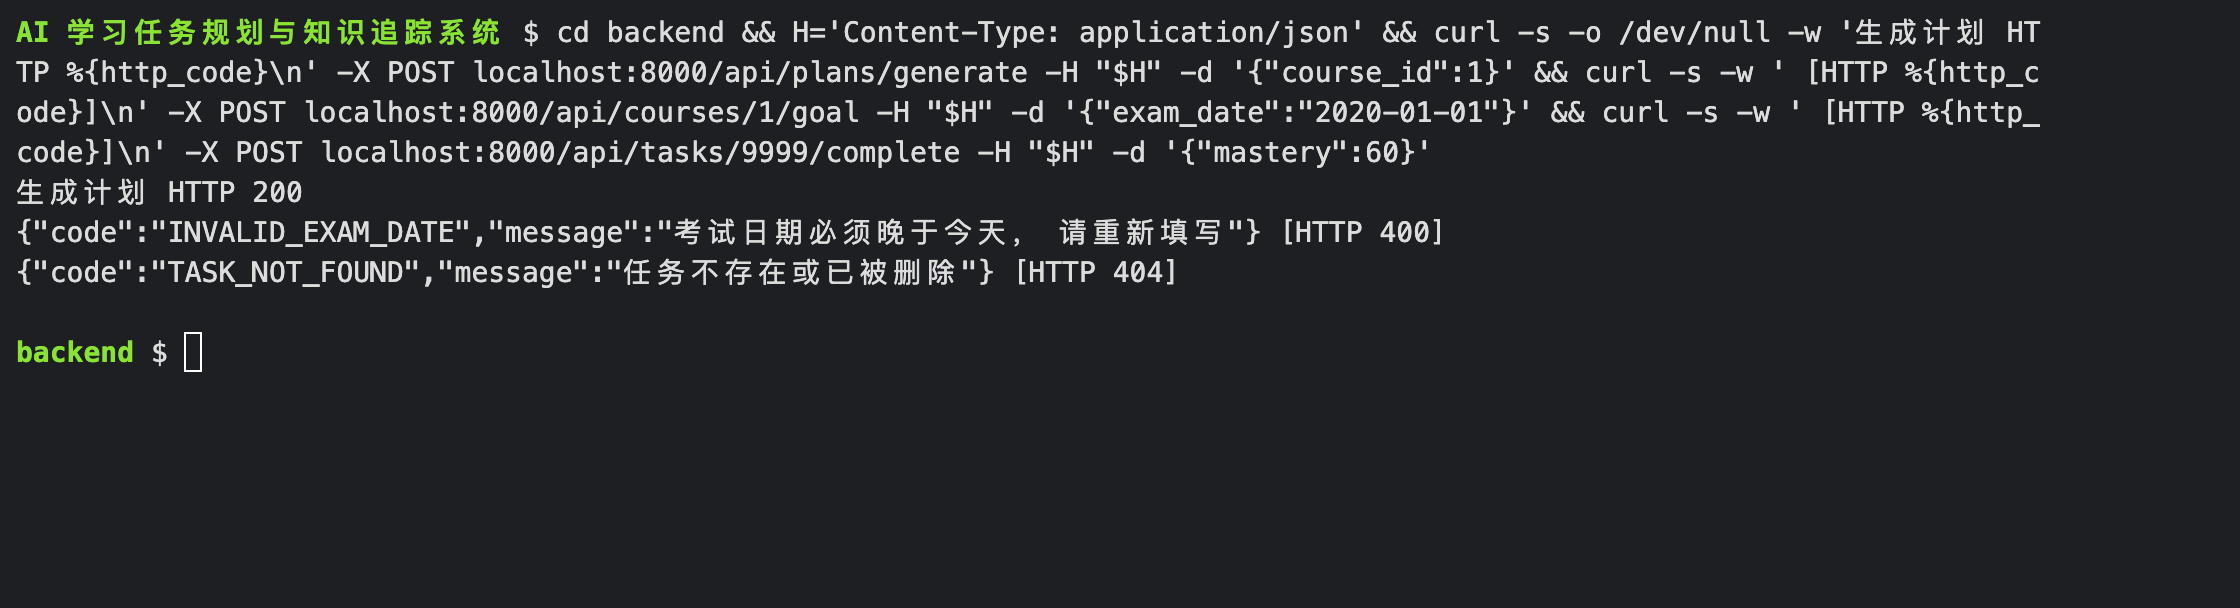
\includegraphics[width=0.96\textwidth]{v02-api.png}\label{fig:api}
\caption{接口返回：正常200、日期错误400、任务不存在404}
\end{figure}

\subsection*{3.4 非AI关键业务闭环}

核心用户故事是“作为本科生，我希望把课程要求转换成可修改的学习计划，以便按时完成任务并了解自己的薄弱知识点”。本次闭环不调用模型服务：计划生成由规则模板完成，掌握度低的知识点优先，任务时长按薄弱程度分配，每天不超过考试目标里的可用时间，并且全部排在考试日期之前。

\begin{table}[H]
\centering
\caption{闭环各步骤与实验3设计的对应关系}
\small
\begin{tabularx}{\textwidth}{p{2.2cm}p{2.1cm}p{3.4cm}X}
\toprule
步骤 & 页面 & 接口与业务模块 & 数据与验收条件 \\
\midrule
创建课程 & 首页 & /api/courses、课程业务 & 写入 courses，重复课程被拒绝 \\
设置考试目标 & 首页 & /api/courses/\{id\}/goal、目标业务 & 写入 exam\_goals，日期必须晚于今天 \\
填写掌握度 & 学习计划页 & /api/courses/\{id\}/points、知识点业务 & 写入 knowledge\_points，掌握度 0—100 \\
生成候选计划 & 学习计划页 & /api/plans/generate、计划业务 & 只返回候选任务，不写库；每天不超可用时间 \\
确认计划 & 学习计划页 & /api/plans/confirm、计划业务 & 写入 study\_plans 和 daily\_tasks，状态 todo \\
完成任务 & 学习进度页 & /api/tasks/\{id\}/complete、任务业务 & 任务改为 done，知识点掌握度按用户确认值更新 \\
调整后续计划 & 学习进度页 & /api/plans/adjust、任务业务 & 未完成任务重新排到考试日期之前 \\
\bottomrule
\end{tabularx}
\end{table}

测试输入取自本人这学期的实际情况：软件工程，考试 2026-11-11，目标 85 分，每天可用 120 分钟，四个知识点掌握度为 30\%、38\%、45\%、62\%。生成结果是 4 个任务，分别排在 10 月 12 日至 10 月 15 日，时长 35、35、30、20 分钟，掌握度最低的软件测试排在最前。完成任务时系统给出建议值 40\%，本人确认后软件测试掌握度从 30\% 更新到 40\%，课程总体掌握度从 44\% 变为 46\%。

\begin{figure}[H]
\centering
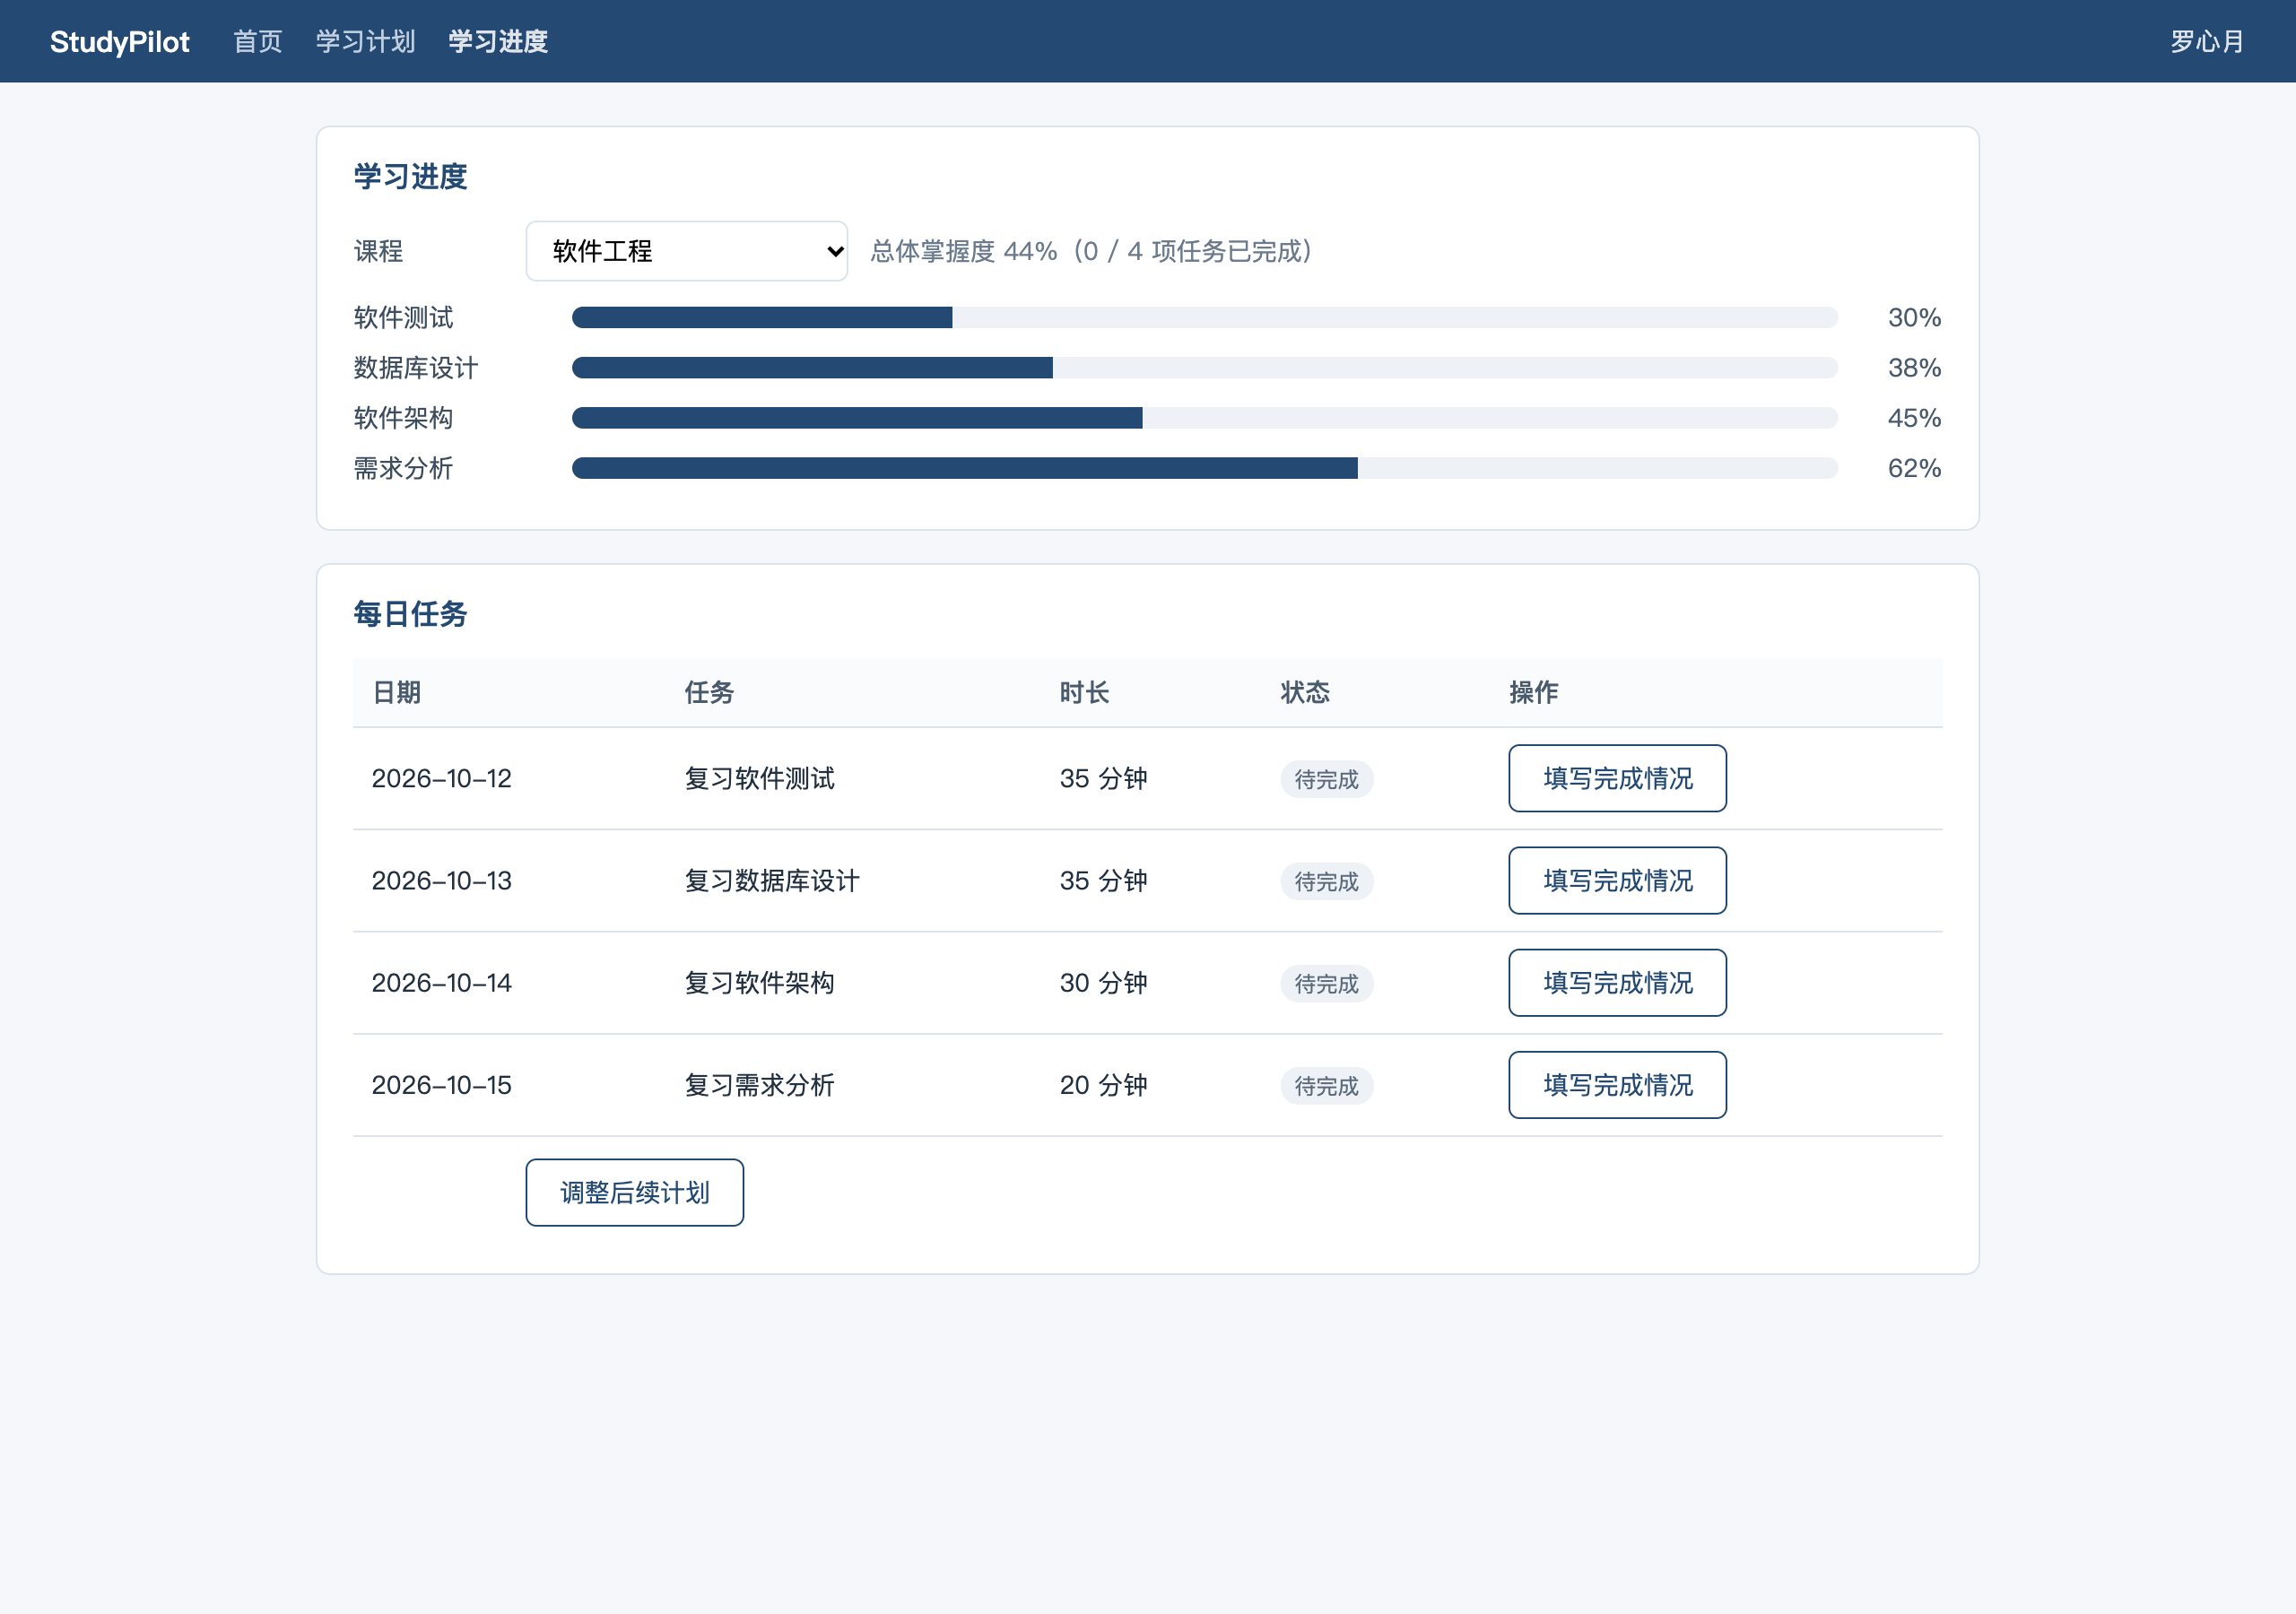
\includegraphics[width=0.88\textwidth]{v02-progress.png}\label{fig:progress}
\caption{学习进度页：掌握度与每日任务}
\end{figure}

\begin{figure}[H]
\centering
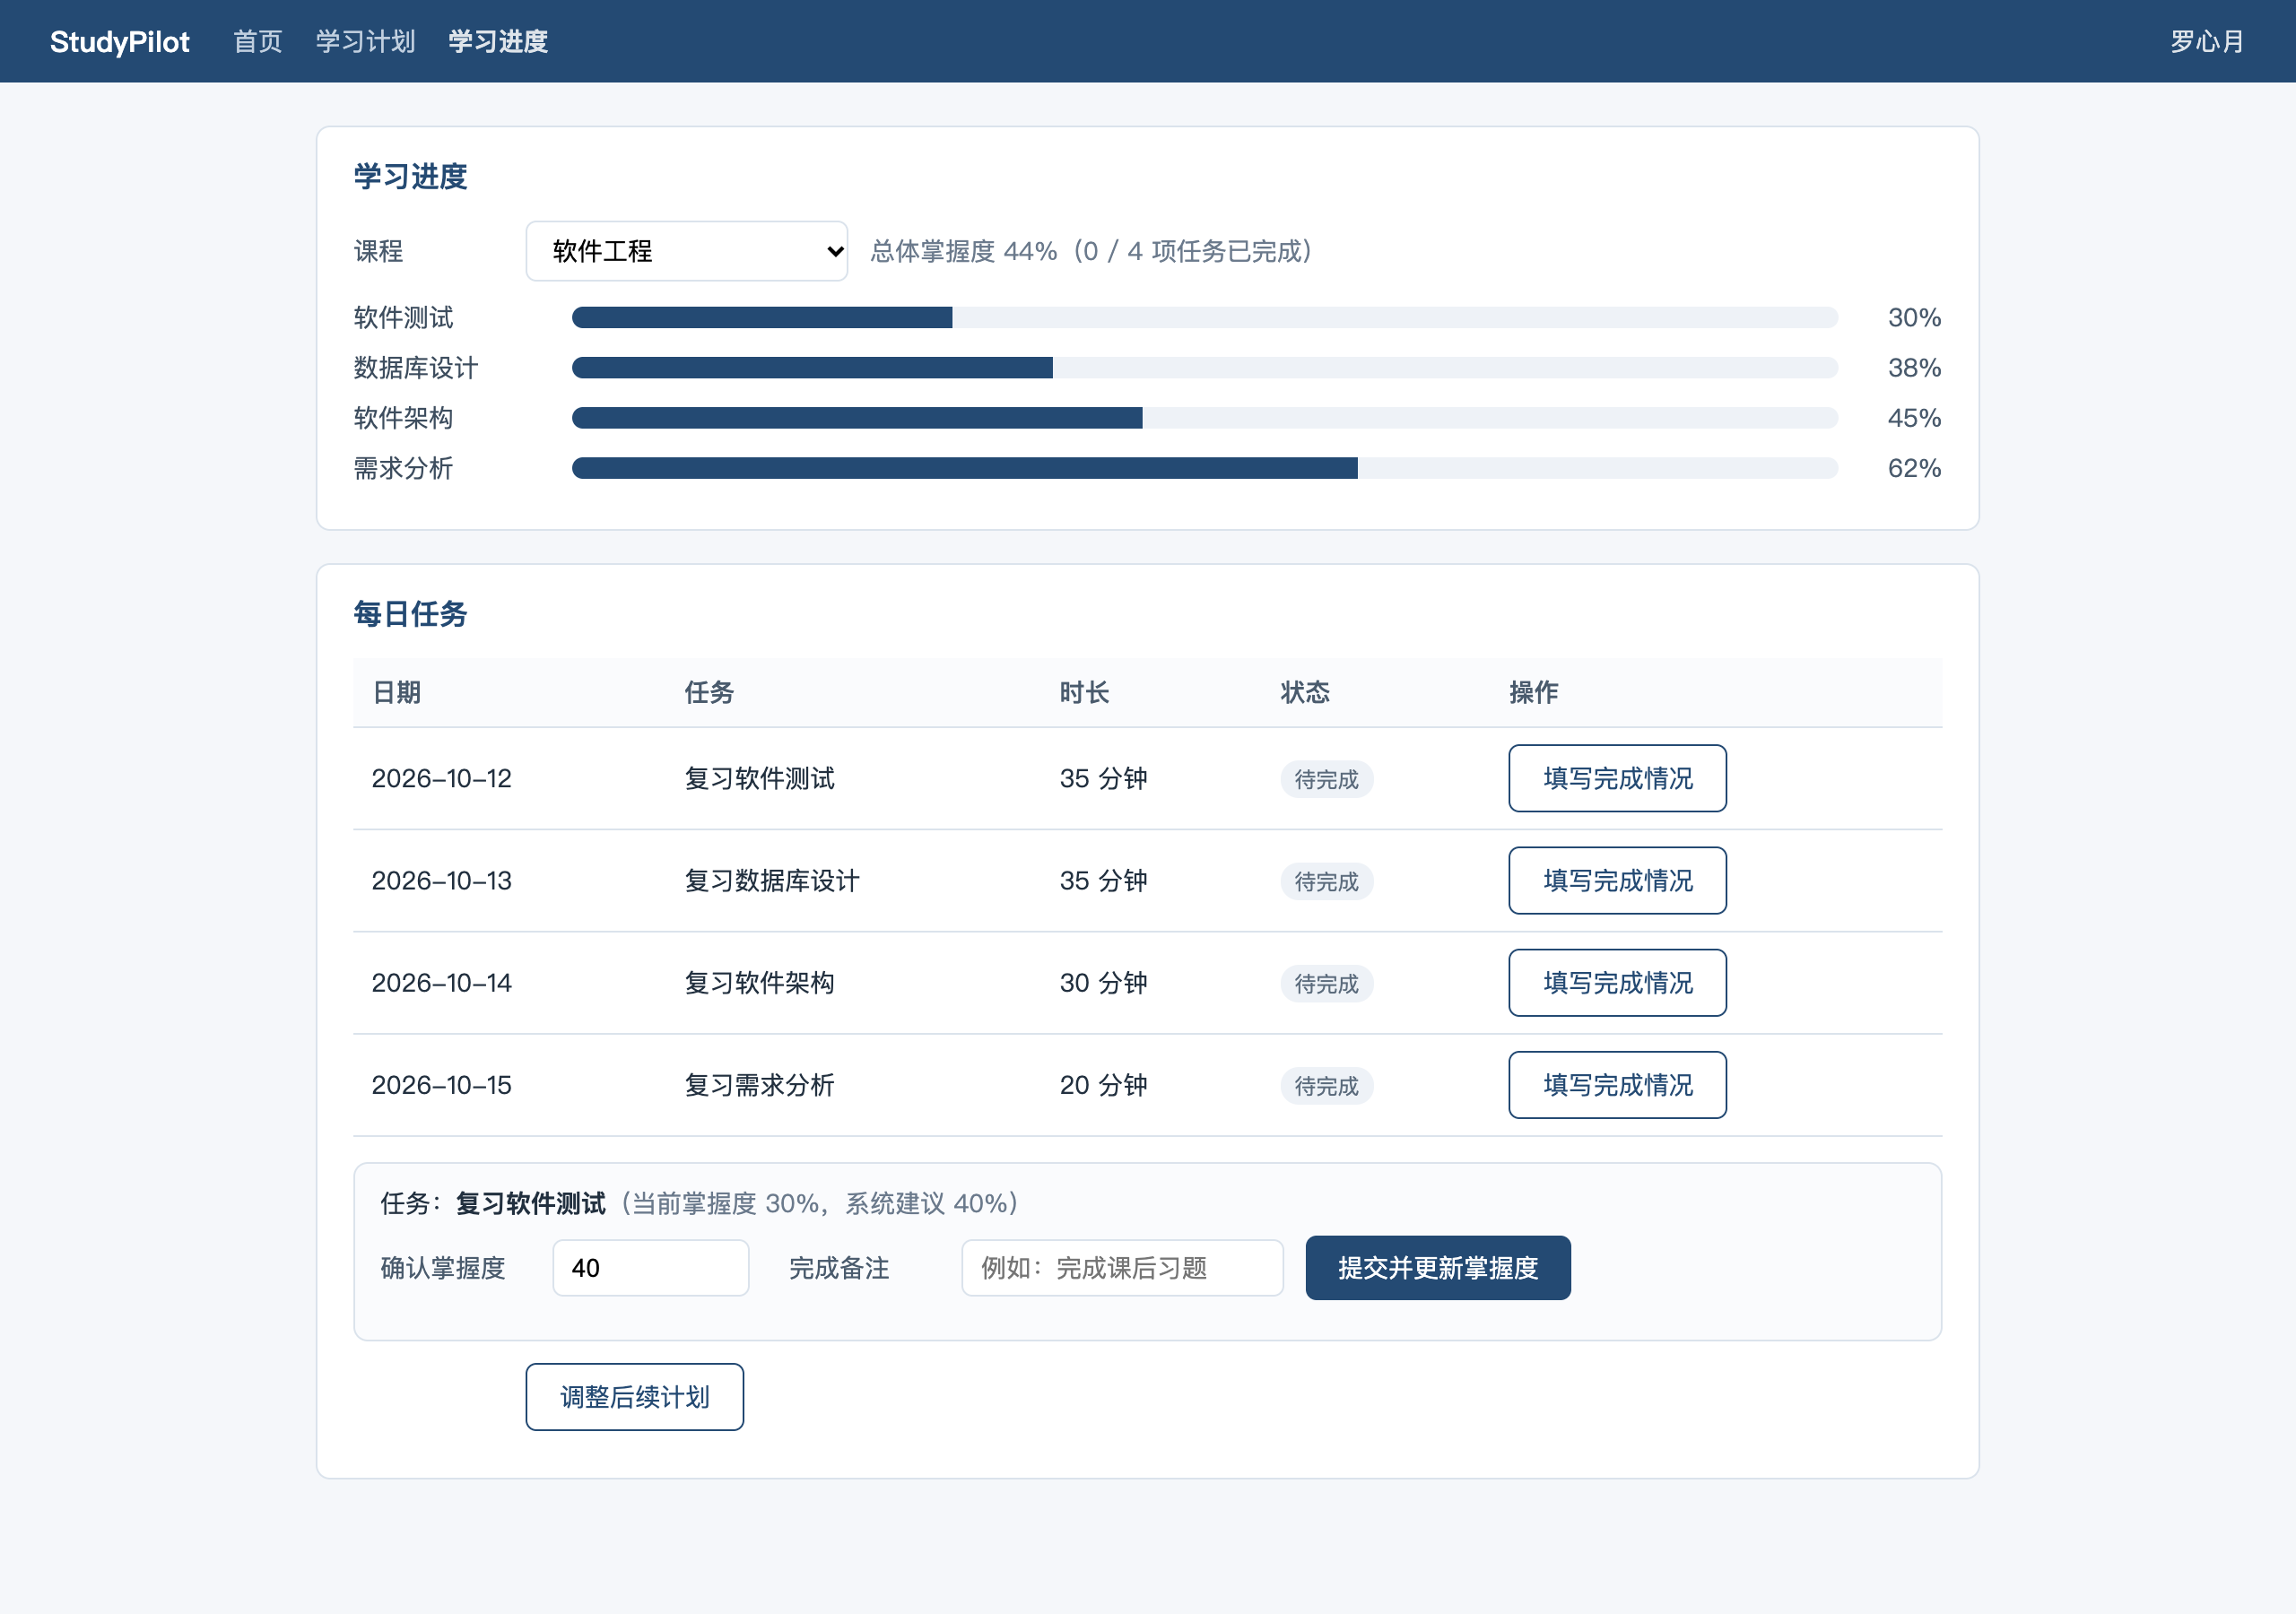
\includegraphics[width=0.88\textwidth]{v02-progress-form.png}\label{fig:form}
\caption{完成情况填写：系统给出建议值，由用户确认}
\end{figure}

\begin{figure}[H]
\centering
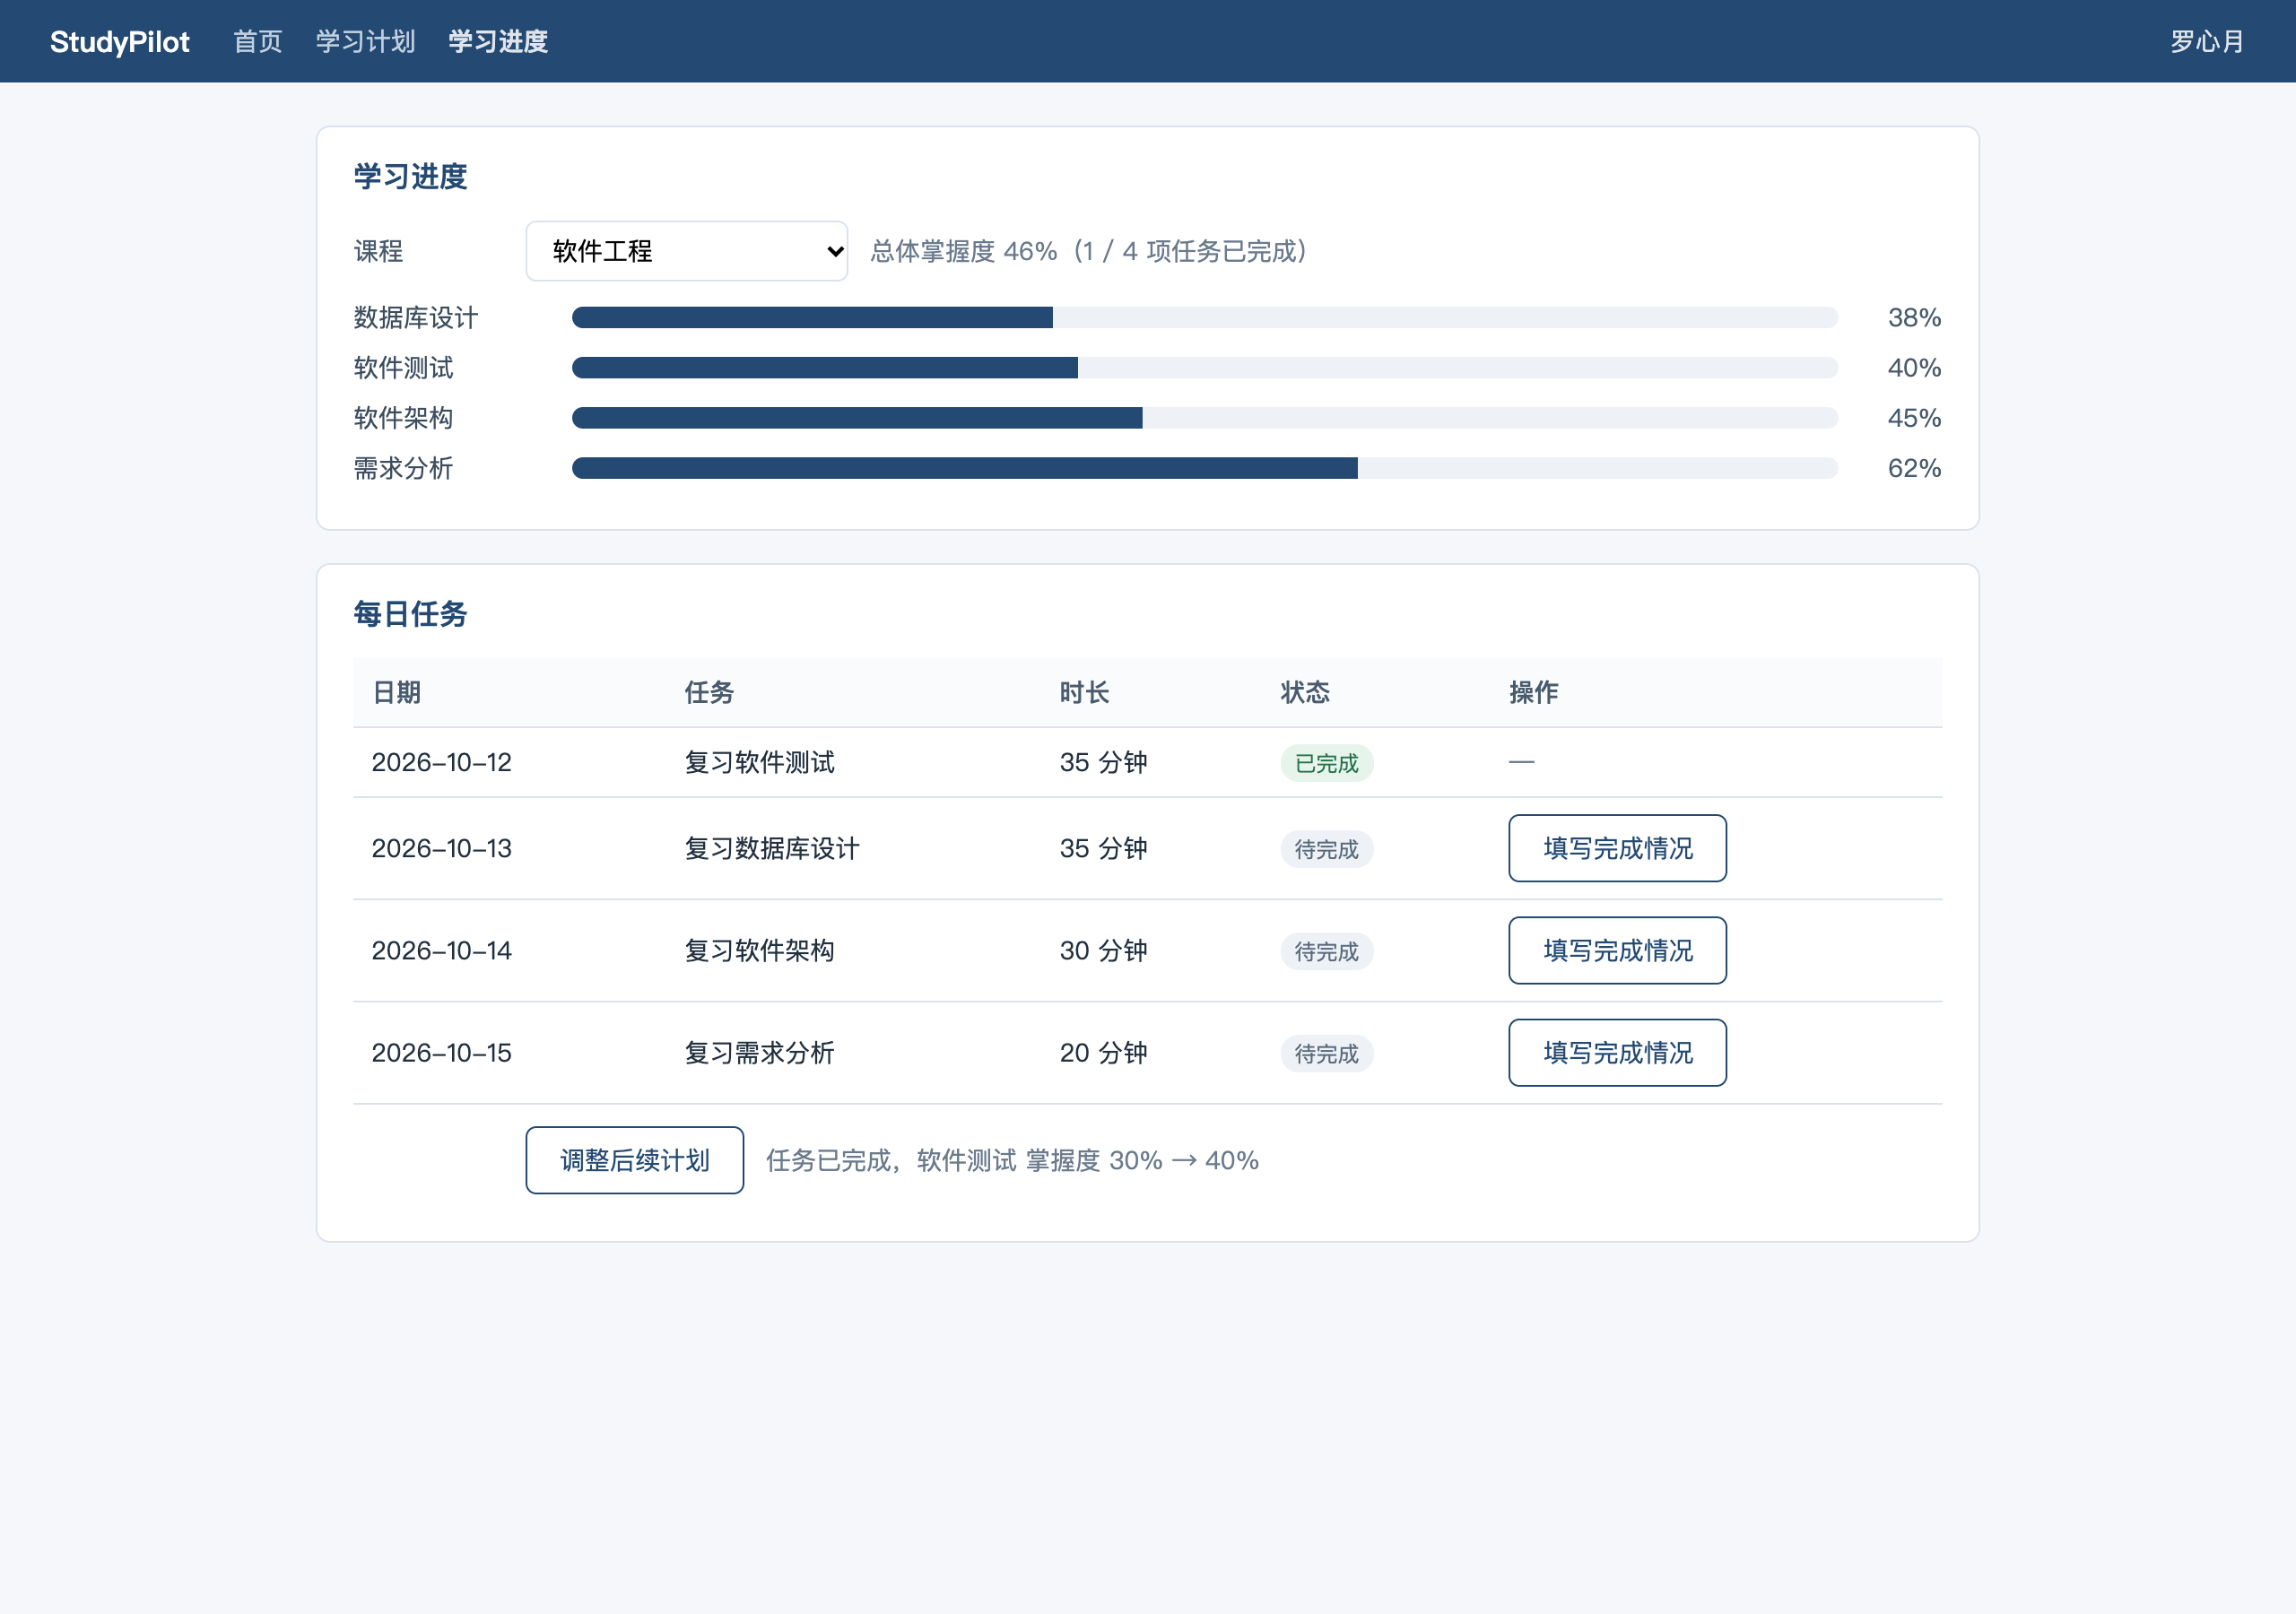
\includegraphics[width=0.88\textwidth]{v02-progress-done.png}\label{fig:done}
\caption{完成结果：掌握度由30\%更新为40\%}
\end{figure}

\begin{figure}[H]
\centering
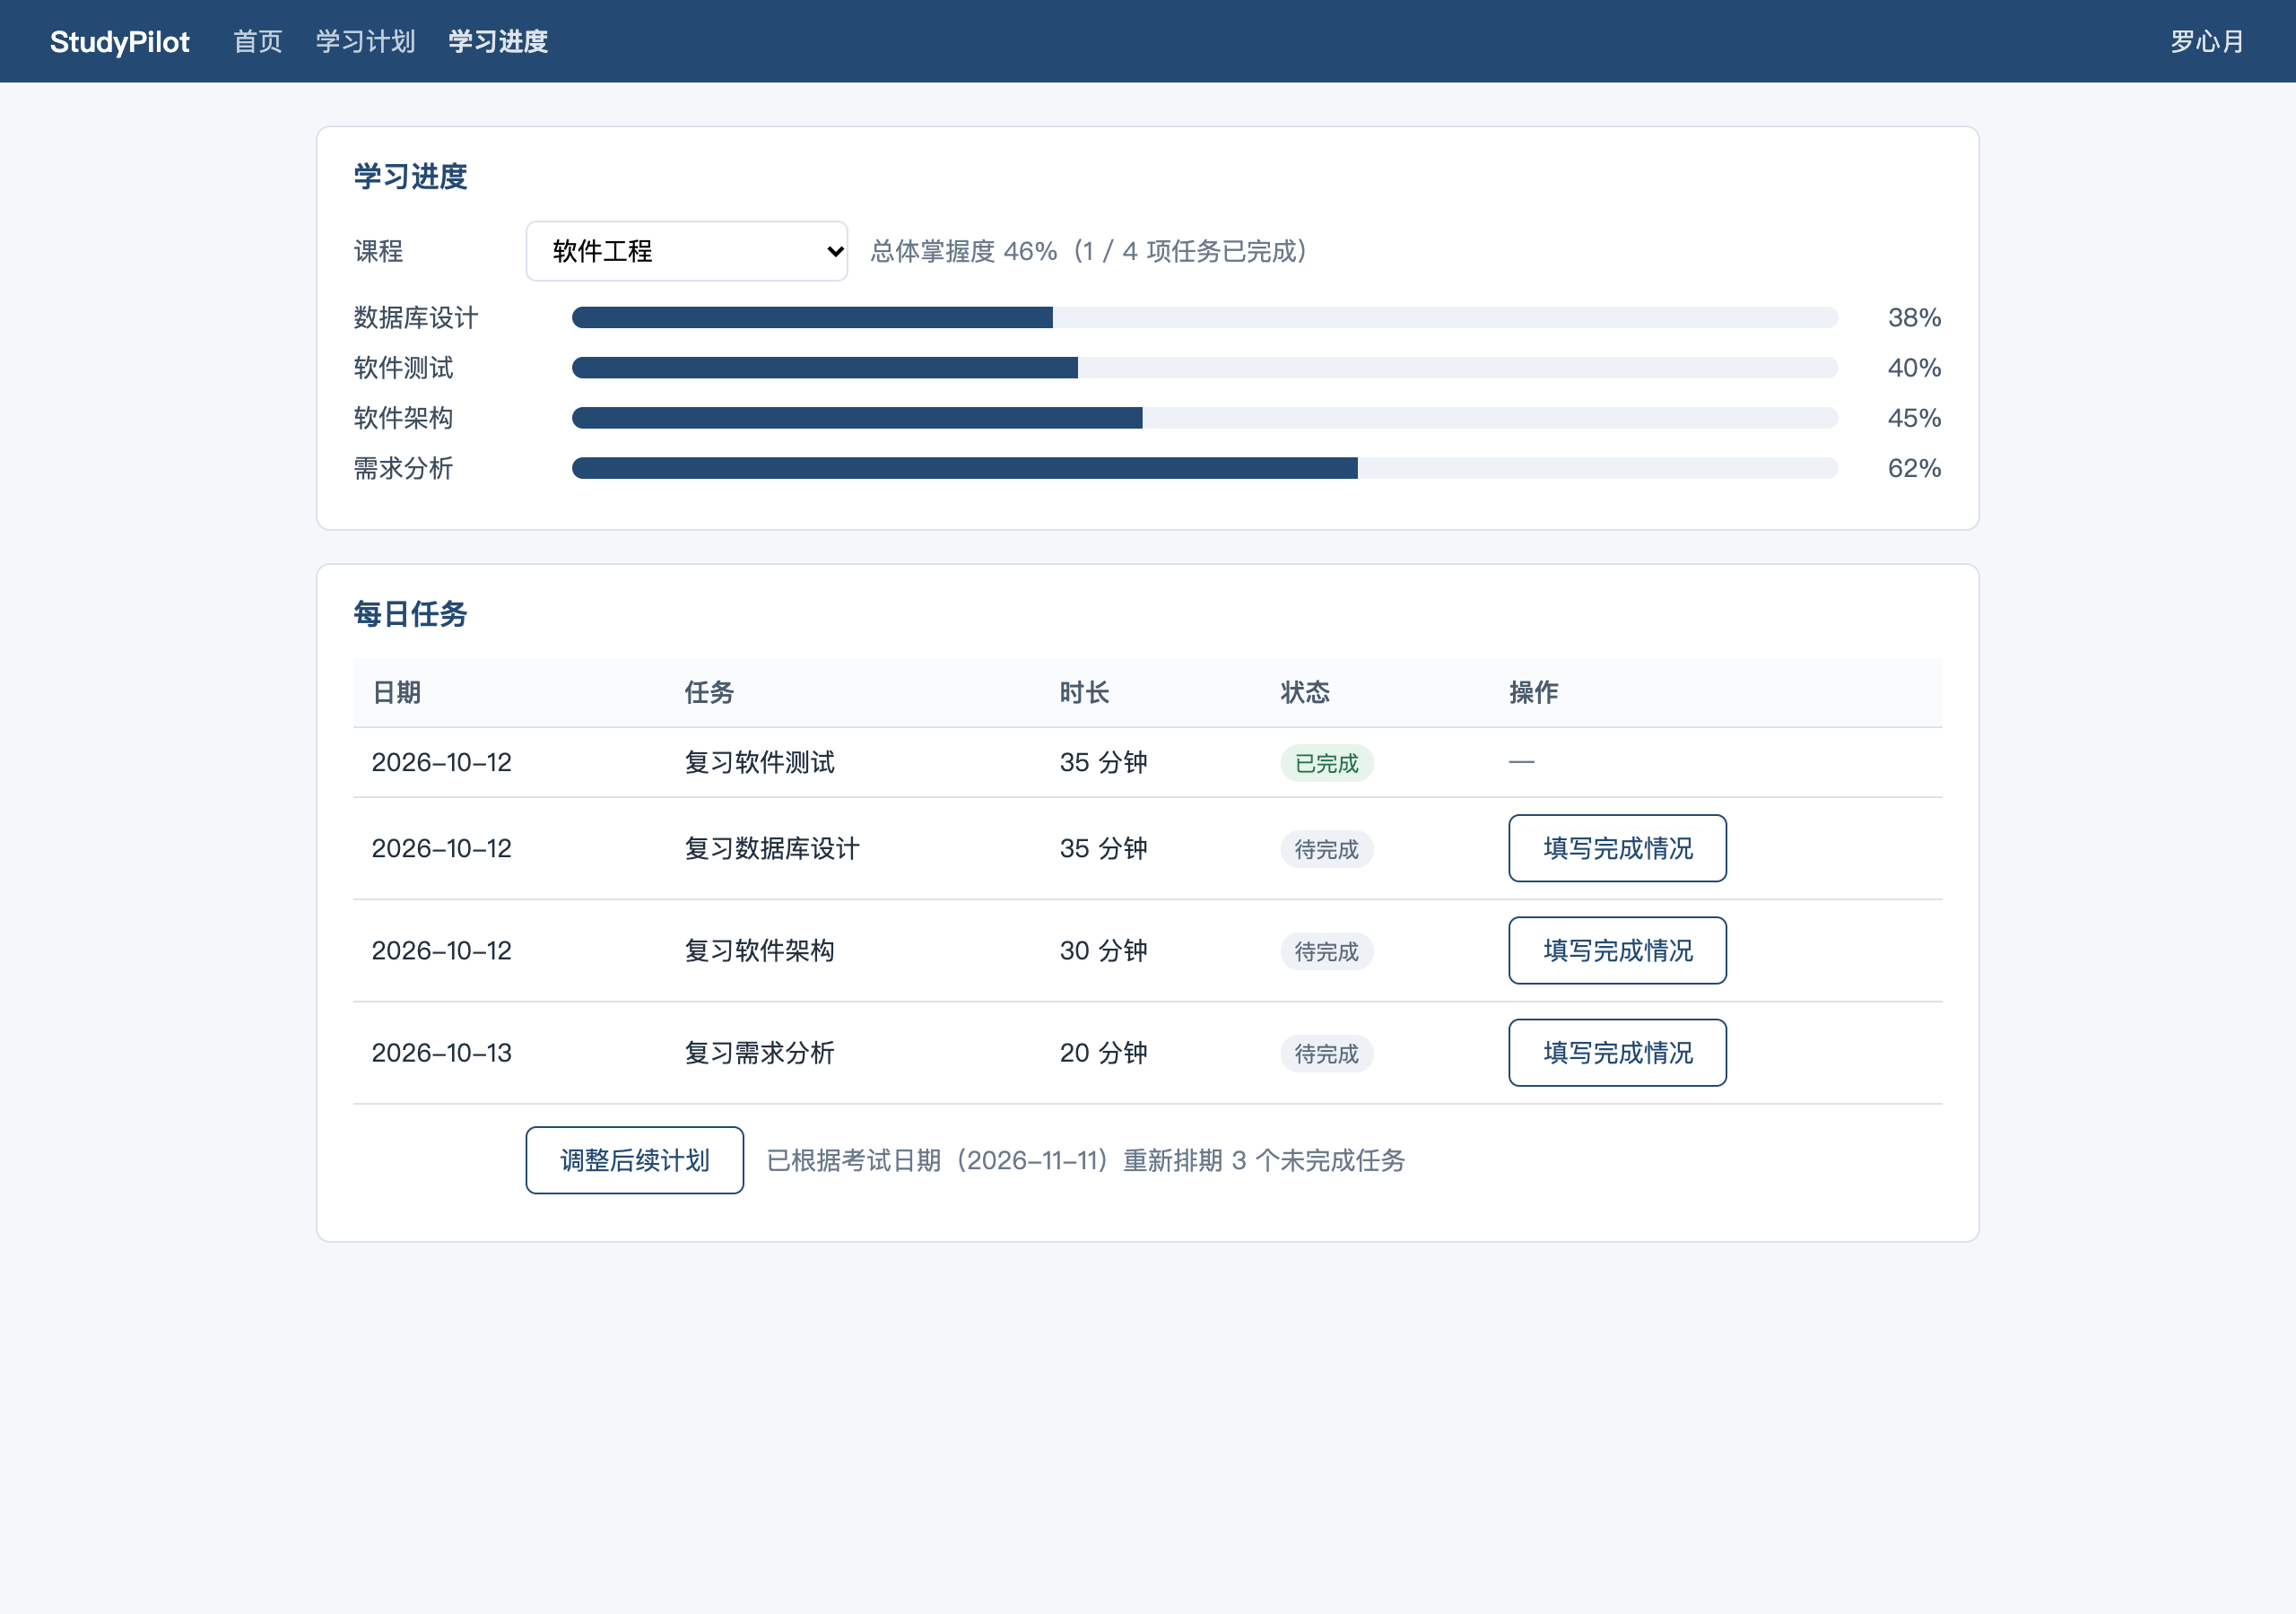
\includegraphics[width=0.88\textwidth]{v02-progress-adjust.png}\label{fig:adjust}
\caption{调整后续计划：未完成任务重新排期}
\end{figure}

\subsection*{3.5 异常处理、日志与基础测试}

异常处理集中在业务层和接口层：业务层抛出带错误码的业务异常，接口层统一转成 JSON，页面直接显示提示文字，程序不会因为一次错误输入中断。

\begin{table}[H]
\centering
\caption{异常处理一览}
\small
\begin{tabularx}{\textwidth}{p{4.6cm}X p{4.4cm}}
\toprule
场景 & 处理方式 & 用户看到的反馈 \\
\midrule
课程名为空 & 业务层拦截，不写库 & 红色提示“课程名称不能为空” \\
课程重名 & 返回 409 & “课程“软件工程”已存在” \\
考试日期早于今天 & 返回 400 & “考试日期必须晚于今天，请重新填写” \\
课程没有知识点 & 返回 400 & “该课程还没有知识点掌握度，请先添加知识点” \\
任务不存在 & 返回 404 & “任务不存在或已被删除” \\
数据库文件损坏 & 捕获 sqlite3 错误，返回 500 并记录异常 & “数据库暂时不可用，请稍后重试” \\
\bottomrule
\end{tabularx}
\end{table}

测试用 pytest 编写，共 10 个用例，每个用例使用独立的临时数据库。初版只有课程接口，所以大部分用例报错；修订版补齐接口和校验后全部通过。

\begin{table}[H]
\centering
\caption{测试用例与两次执行结果}
\scriptsize
\begin{tabularx}{\textwidth}{p{0.6cm}p{2.9cm}p{2.6cm}p{2.4cm}X p{1.3cm}}
\toprule
编号 & 用例 & 预期结果 & 初版(v0.1)结果 & 修复内容 & 复测结果 \\
\midrule
T1 & 创建课程 & 返回 201 并能查到 & 失败：返回 409 & 启动不再自动写样例课程，改用 seed 脚本；测试用临时库 & 通过 \\
T2 & 重复课程名 & 返回 409 与提示 & 报错：创建课程就冲突 & 同上，重名校验保留在业务层 & 通过 \\
T3 & 课程名为空 & 返回 400，列表为空 & 失败：列表中有样例课程 & 同上 & 通过 \\
T4 & 考试日期早于今天 & 返回 400 & 报错：接口不存在 & 新增考试目标接口与日期校验 & 通过 \\
T5 & 没有知识点就生成计划 & 返回 400 与提示 & 报错：接口不存在 & 新增生成接口；AI初稿此处除零，改为先校验 & 通过 \\
T6 & 生成计划规则 & 覆盖全部知识点、不超可用时间、早于考试 & 报错：接口不存在 & 新增规则模板：按掌握度分配时长并分散排期 & 通过 \\
T7 & 确认计划 & 计划已确认，任务写入 & 报错：接口不存在 & 新增确认接口，确认时覆盖旧任务 & 通过 \\
T8 & 完成任务并更新掌握度 & 任务完成，掌握度更新 & 报错：接口不存在 & 新增任务接口，掌握度按用户确认值写入 & 通过 \\
T9 & 完成不存在的任务 & 返回 404 & 报错：接口不存在 & 新增任务查询与 404 处理 & 通过 \\
T10 & 数据库不可用 & 返回 500 与统一提示 & 失败：直接抛出 DatabaseError & 数据访问层捕获 sqlite3 错误，转成业务异常并写日志 & 通过 \\
\bottomrule
\end{tabularx}
\end{table}

\begin{figure}[H]
\centering
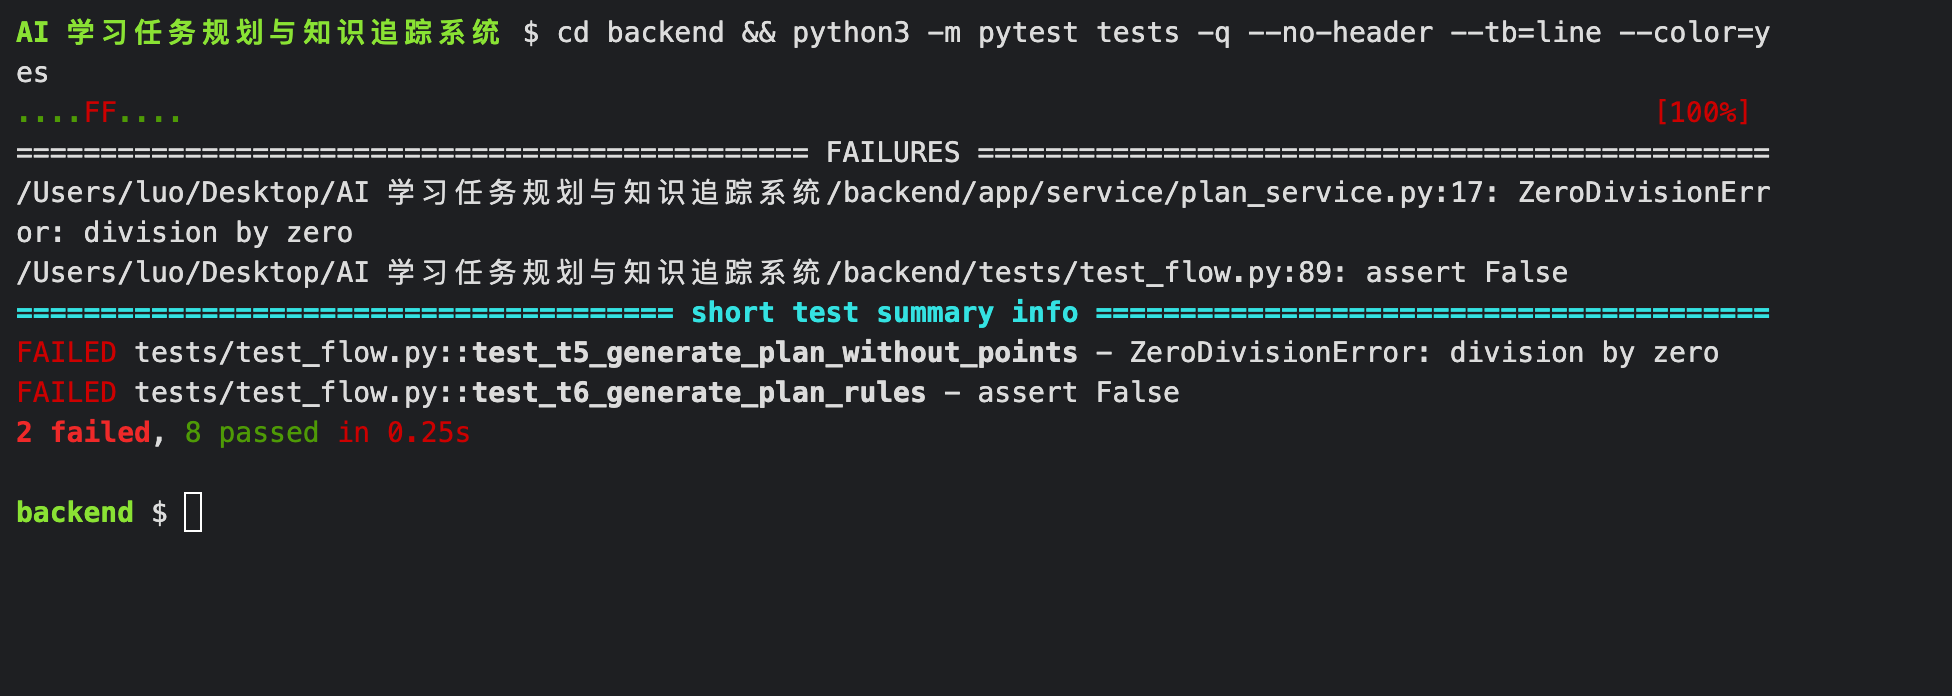
\includegraphics[width=0.96\textwidth]{v02-draft-test.png}\label{fig:drafttest}
\caption{初版与AI初稿的测试结果：2个用例失败}
\end{figure}

\begin{figure}[H]
\centering
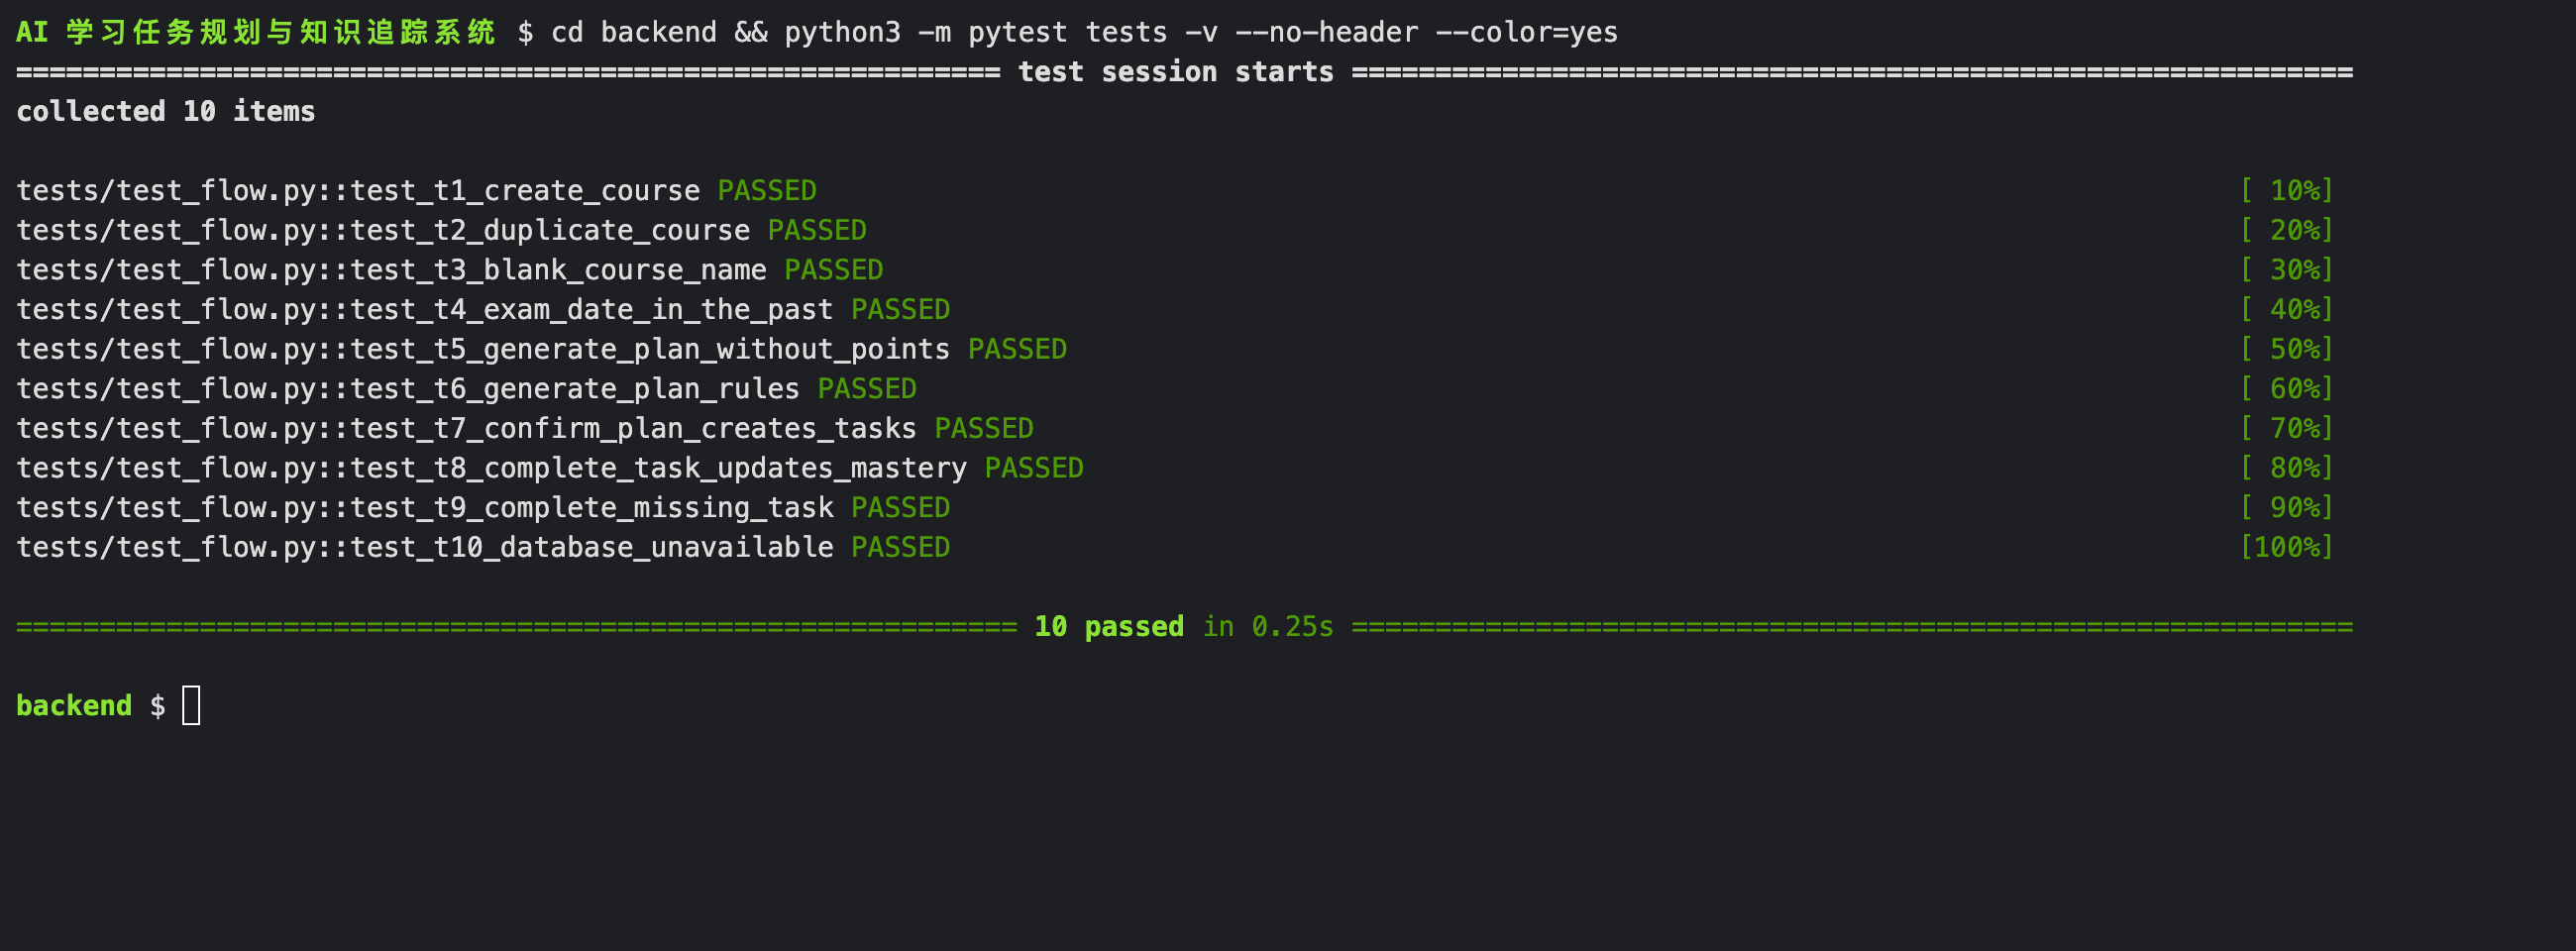
\includegraphics[width=0.96\textwidth]{v02-tests-pass.png}\label{fig:tests}
\caption{修订版复测：10个用例全部通过}
\end{figure}

日志写在 \texttt{backend/logs/app.log}，同时打印到控制台。记录内容包括：启动时的数据库位置、样例数据写入、每次业务操作的结果（如创建课程、生成计划、确认计划、完成任务）、业务异常的请求方法与错误码，以及未处理异常的完整堆栈。下面是完成任务不存在时接口返回 404 的日志，可以看到错误码 \texttt{TASK\_NOT\_FOUND} 和前面的数据库异常堆栈。

\begin{figure}[H]
\centering
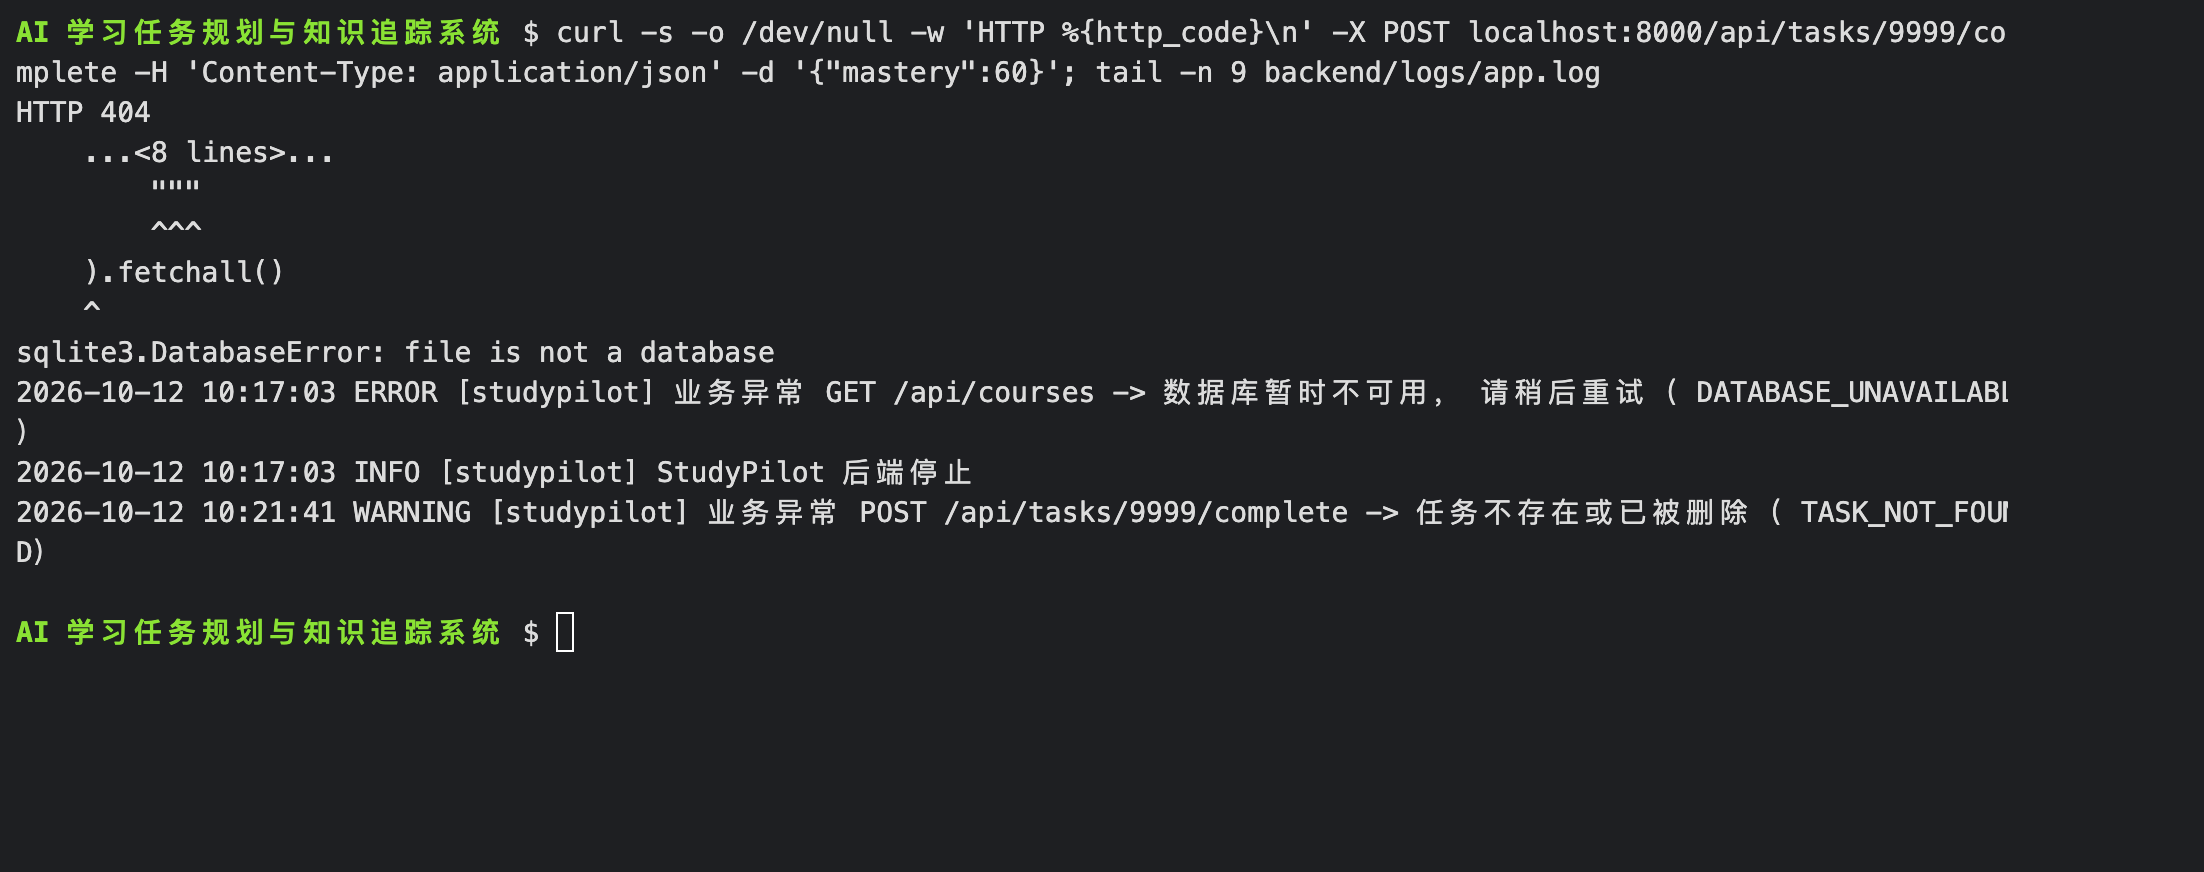
\includegraphics[width=0.96\textwidth]{v02-logs.png}\label{fig:logs}
\caption{运行日志：业务异常与数据库异常堆栈}
\end{figure}

\begin{figure}[H]
\centering
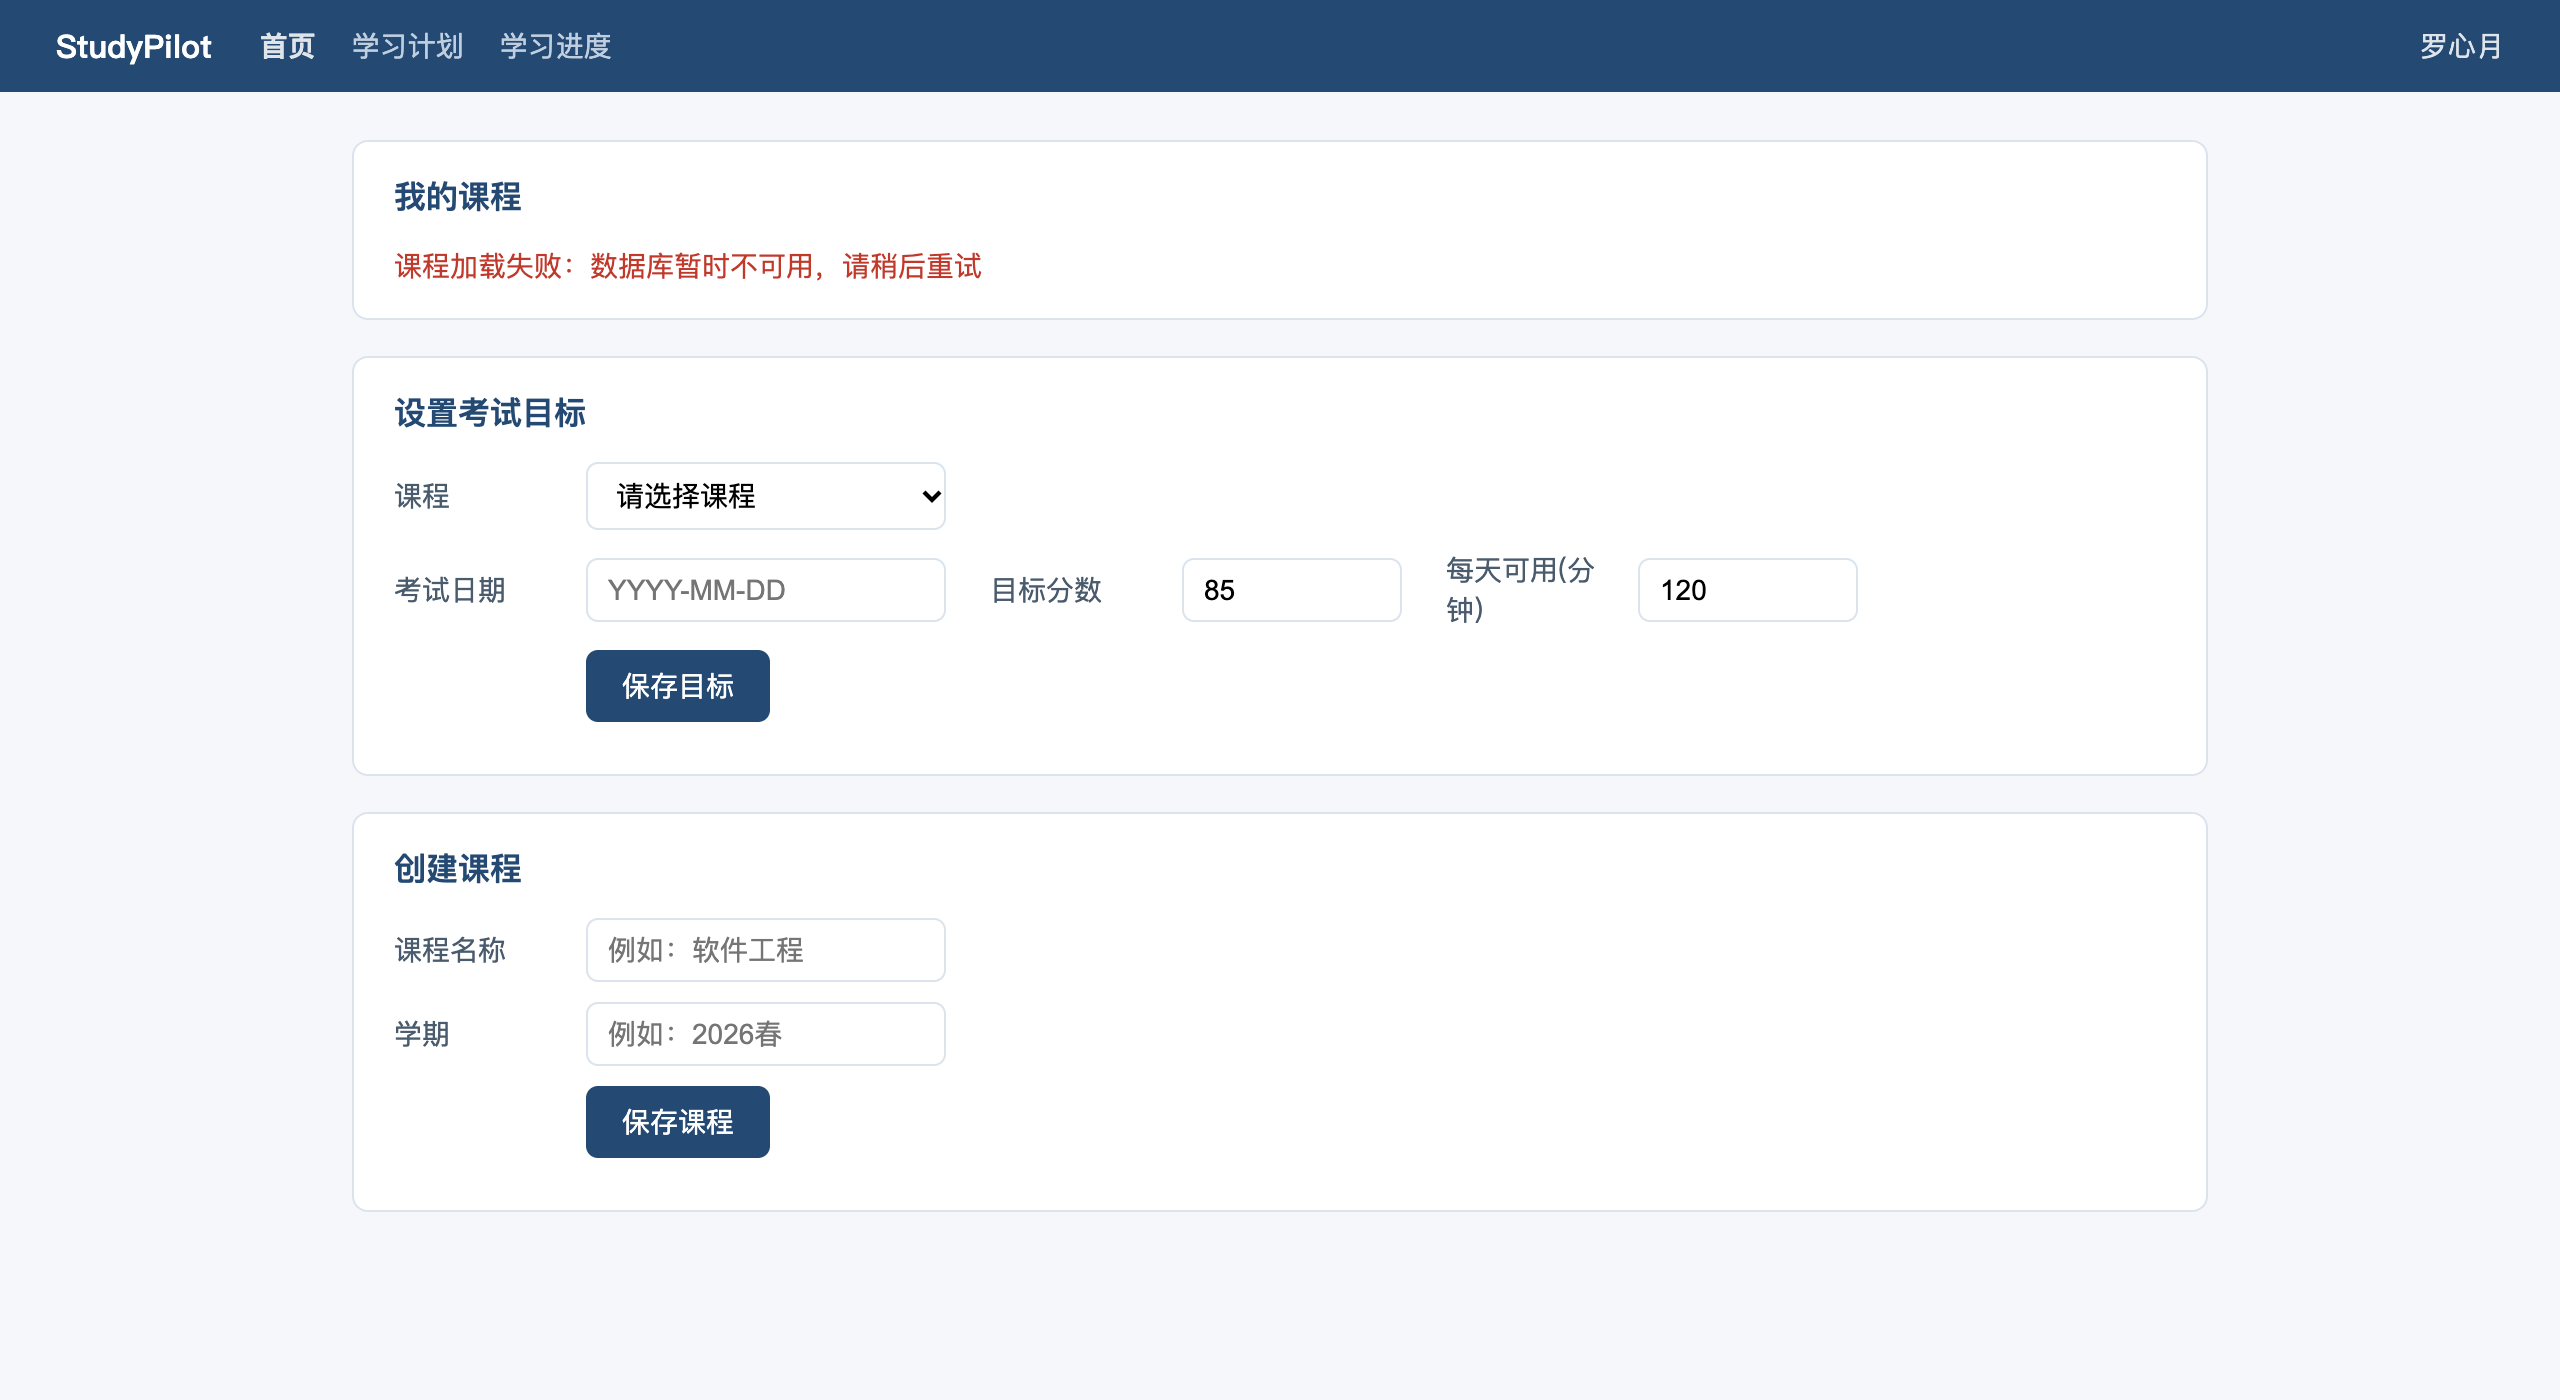
\includegraphics[width=0.8\textwidth]{v02-db-error.png}\label{fig:dberror}
\caption{数据库不可用时页面给出统一提示}
\end{figure}

\subsection*{3.6 AI辅助编码审查}

\textbf{任务}：让AI生成“学习计划生成服务”的初稿，输入课程编号，输出候选任务列表，要求按知识点拆分并给出时长和日期。\\

\textbf{AI建议}（图\ref{fig:draftcode}）：遍历知识点，每个任务固定 45 分钟、日期都取今天，用知识点平均掌握度拼一句说明文字，接口里直接标 \texttt{generator="llm"}。\\

\textbf{采用的内容}：按知识点拆分任务、任务带上知识点编号和说明文字、先返回候选结果由用户确认后再保存。\\

\textbf{拒绝或修改的内容}：
\begin{itemize}
  \item 固定 45 分钟、全部排在同一天：不符合“每天可用 120 分钟”的设定，改为按掌握度薄弱程度分配时长，并按天分散。
  \item 忽略考试日期：改为只使用考试日期之前、最多 7 天的可用日期，排不下时给出提示。
  \item 没有校验：知识点为空时做除法会抛 \texttt{ZeroDivisionError}，改为先校验知识点和考试目标并返回 400 提示。
  \item 无用依赖：初稿 import 了 \texttt{plan\_repo}、\texttt{ai\_service} 和 \texttt{BusinessError} 都没有用到，已删除或改成真正使用。
  \item 不存在的实现：初稿返回 \texttt{generator="llm"}，但代码里没有任何模型调用，属于写了不存在的接口；改为按实际情况返回生成方式和模型服务是否可用。
  \item 安全问题：SQL 全部使用参数化查询，没有拼接字符串；模型密钥只从环境变量 \texttt{LLM\_API\_KEY} 读取，不写进代码和仓库。
\end{itemize}

\textbf{测试验证}：修改前 T5、T6 失败（图\ref{fig:drafttest}），修改后 10 个用例全部通过（图\ref{fig:tests}），改动内容见图\ref{fig:fix}。局限是规则模板只按掌握度和可用时间排期，不考虑课程难度和用户偏好，知识点较多时后面的知识点可能排不进考试前的天数，需要在后续版本补充。

\begin{figure}[H]
\centering
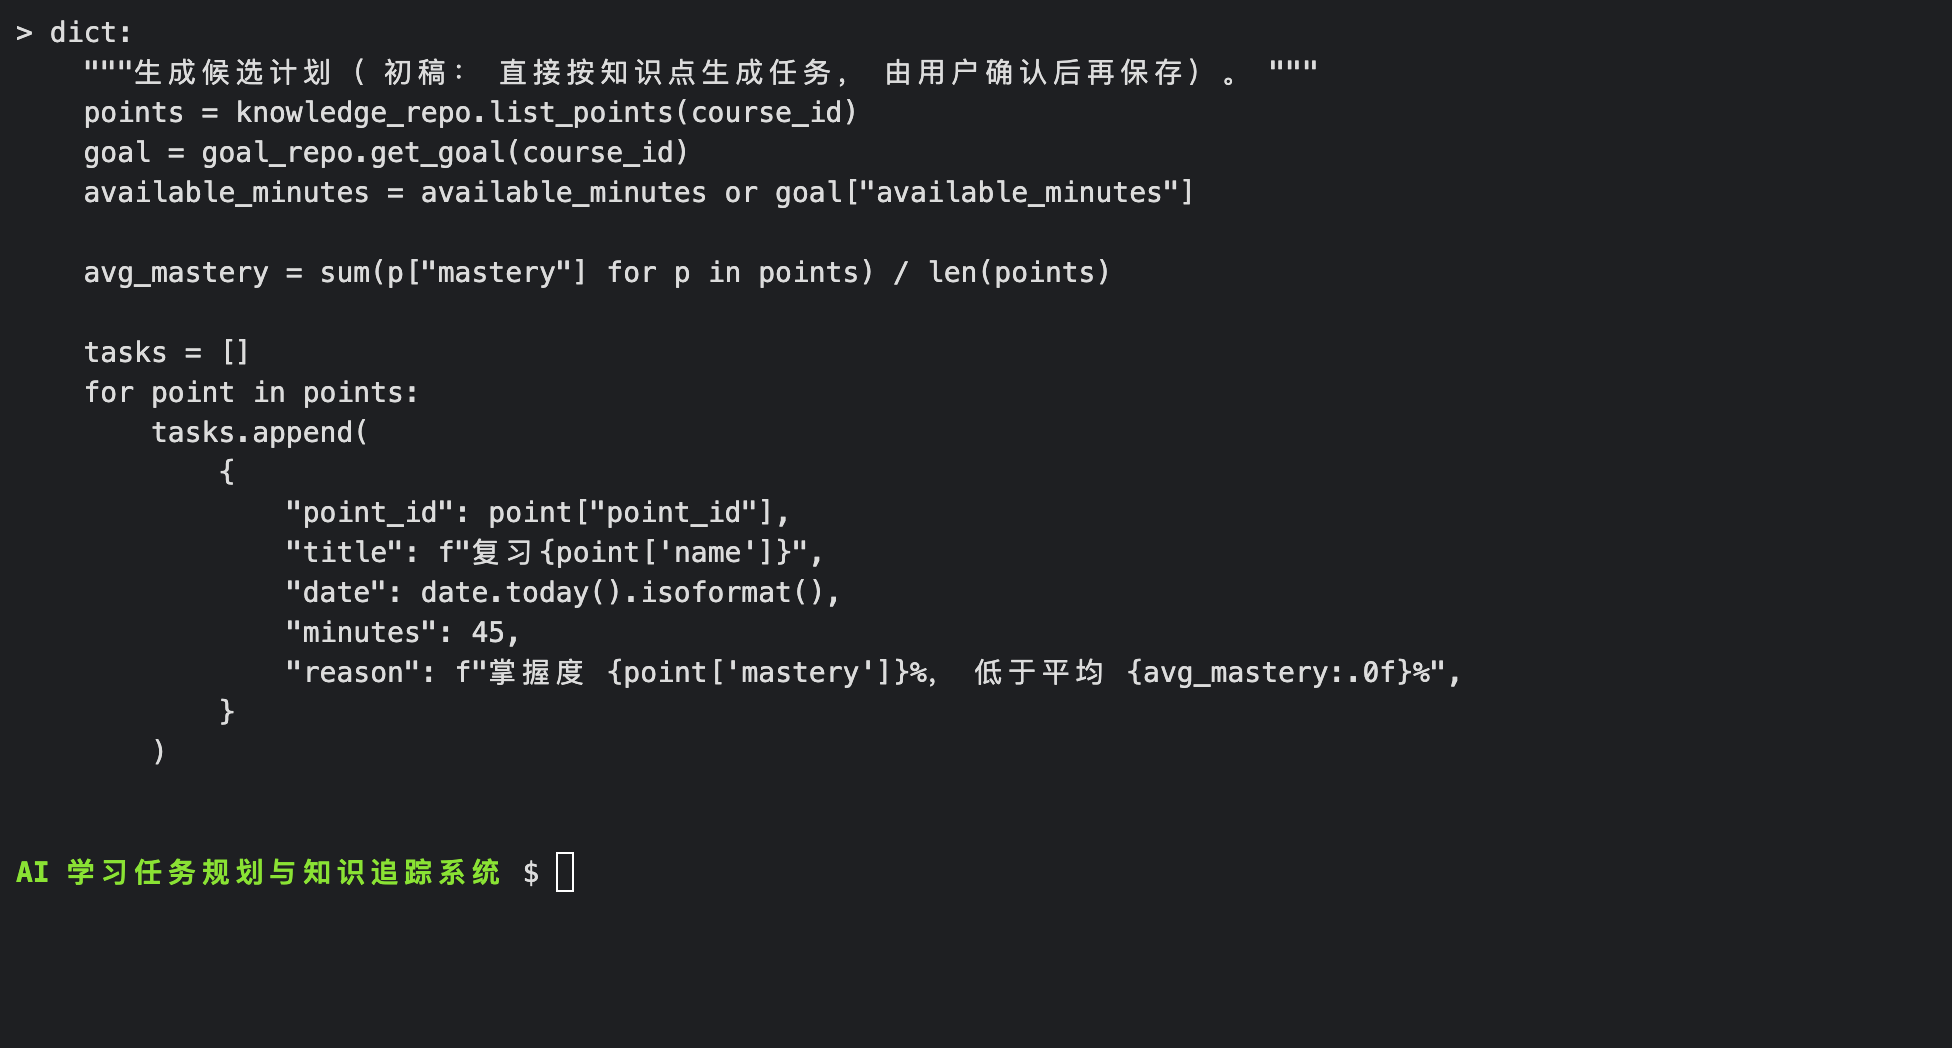
\includegraphics[width=0.92\textwidth]{v02-draft-code.png}\label{fig:draftcode}
\caption{AI初稿代码：固定45分钟、忽略考试日期、未做空数据校验}
\end{figure}

\begin{figure}[H]
\centering
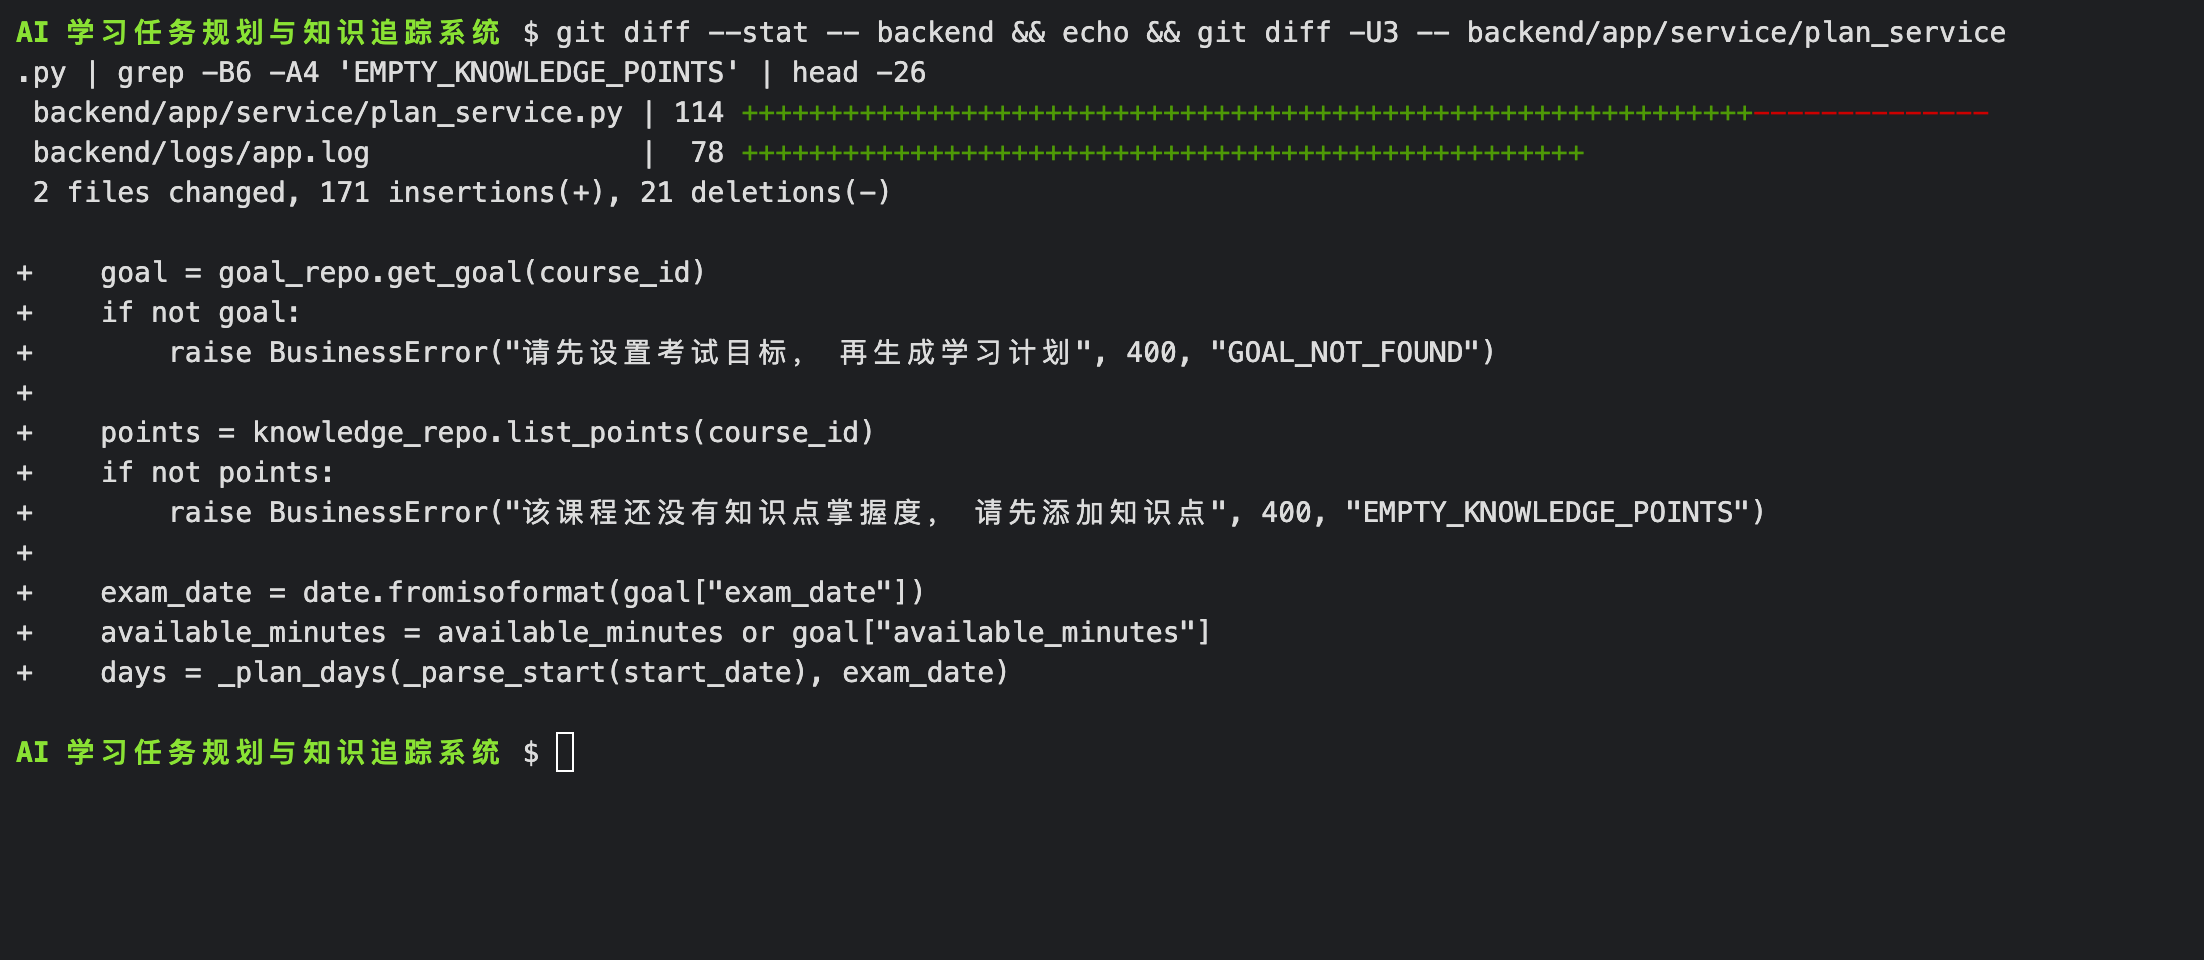
\includegraphics[width=0.96\textwidth]{v02-fix-hunk.png}\label{fig:fix}
\caption{人工修正：补充考试目标与知识点校验（diff）}
\end{figure}

\subsection*{3.7 版本保存与推送}

代码和报告都提交到 GitHub 仓库 \url{https://github.com/luohao711/StudyPilot}，初版和修订版分别对应 tag \texttt{v0.1}（cee3baa）和 \texttt{v0.2}（c390c38）。

\begin{figure}[H]
\centering
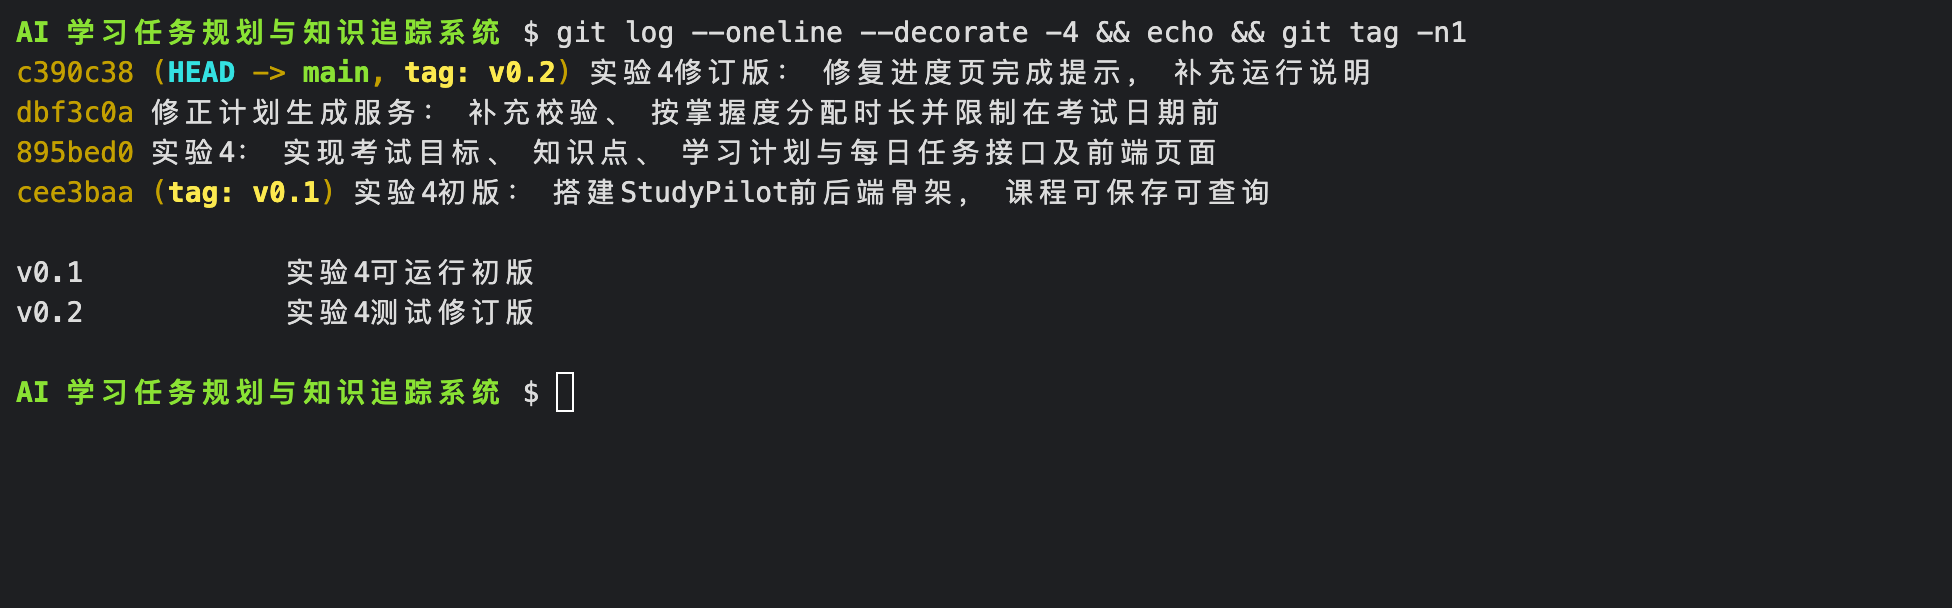
\includegraphics[width=0.96\textwidth]{v02-push.png}\label{fig:push}
\caption{推送到GitHub的记录}
\end{figure}

\begin{figure}[H]
\centering
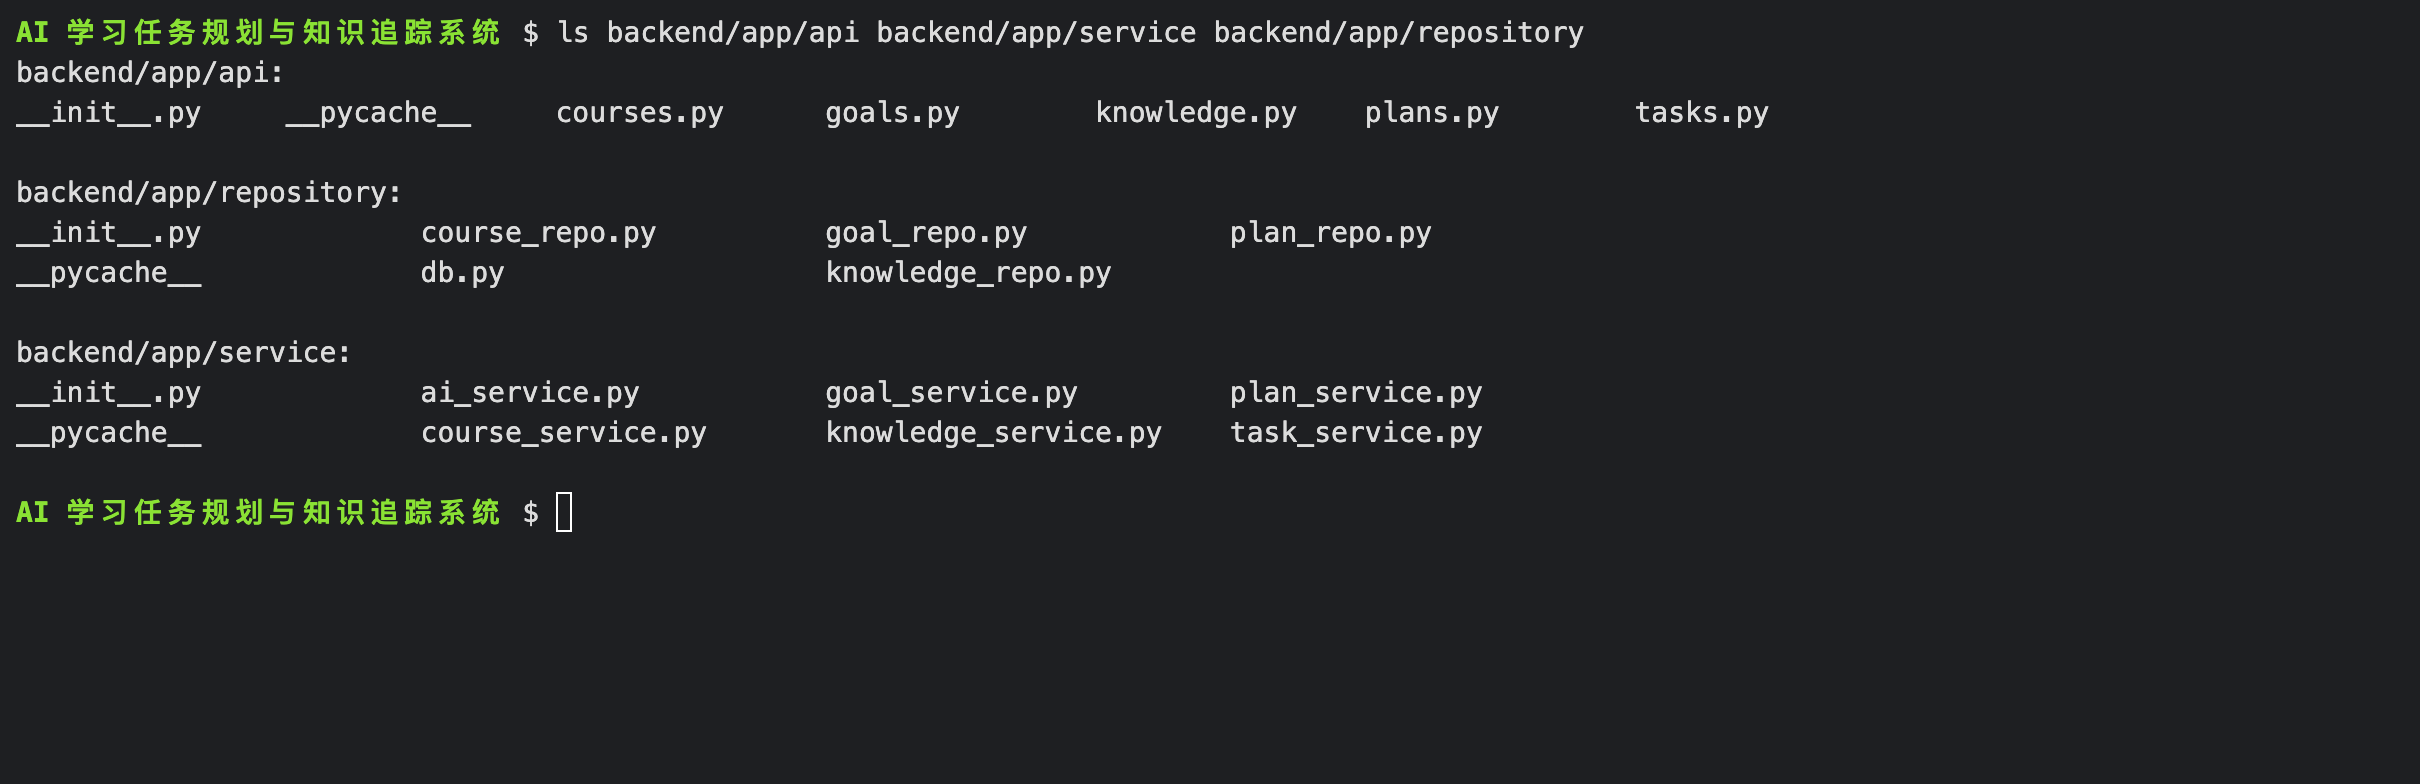
\includegraphics[width=0.9\textwidth]{v02-github.png}\label{fig:github}
\caption{StudyPilot仓库页面}
\end{figure}

\section*{4. 实验小结}

本次完成了 StudyPilot 的基础功能：后端用 FastAPI 分层实现，数据存 SQLite，前端用 Vue 3 做了首页、学习计划页和学习进度页，把实验3设计的核心流程真正跑通了一遍。计划生成没有调用模型服务，而是用规则模板降级完成，模型服务配置好后可以在同一个入口替换。

过程中主要遇到三个问题。一是初版启动时会自动写入样例课程，测试之间互相干扰，改为启动只建表、样例数据用脚本单独写入。二是 AI 初稿的计划生成既没有校验也会忽略考试日期，跑测试时出现除零错误，按掌握度重新分配时长并加上日期限制后通过。三是进度页一开始把完成提示清掉了，用户看不到掌握度的变化，调整了提示和刷新的顺序。

测试共 10 个用例，覆盖正常流程、无效输入、数据不存在和数据库不可用，修订版全部通过。遗留的问题是：知识点的掌握度只靠用户自评，缺少根据任务完成情况自动建议的依据；模型服务接入后还需要补充结果校验，防止模型返回的日期或时长不合法。

\end{document}
